\documentclass[12pt,letterpaper]{article}

% --- 1. CONFIGURACIÓN DE IDIOMA Y CARACTERES ---
\usepackage[utf8]{inputenc}
\usepackage[T1]{fontenc}
\usepackage[spanish, es-nodecimaldot, es-noquoting]{babel}
\usepackage{csquotes}
\usepackage{mathpazo}          % Palatino para texto y matemáticas
\usepackage{textcomp}          % Complemento de texto
\usepackage{microtype}

% --- 2. GEOMETRÍA ---
\usepackage[margin=2.5cm, headheight=14pt]{geometry}

% --- 3. ESPACIADO ENTRE PÁRRAFOS ---
\setlength{\parskip}{0.6em}
\setlength{\parindent}{0pt}

% --- 4. MATEMÁTICAS ---
\usepackage{amsmath,amssymb}

% --- 5. TABLAS Y GRÁFICOS ---
\usepackage{booktabs}
\usepackage{array}
\usepackage{colortbl}
\usepackage{xcolor}
\usepackage{graphicx}
\usepackage{float}
\usepackage{wrapfig}
\usepackage{pifont}

% --- 6. CAJAS Y ENTORNOS ---
\usepackage{tcolorbox}
\tcbuselibrary{skins,breakable}

% --- 7. ENCABEZADOS Y PIES ---
\usepackage{fancyhdr}
\pagestyle{fancy}
\fancyhf{}
\fancyhead[L]{\small\textsc{Optimización Inteligente}}
\fancyhead[R]{\small\textsc{MIAAD \textcolor{uacjgray}{\textbullet} UACJ}}
\fancyfoot[C]{\thepage}
\renewcommand{\headrulewidth}{0.4pt}

% --- 8. HIPERVÍNCULOS ---
\usepackage{hyperref}
\hypersetup{colorlinks=true, linkcolor=blue!60!black, urlcolor=blue!60!black, citecolor=blue!60!black}

% --- 9. COLORES PERSONALIZADOS ---
\definecolor{headerblue}{HTML}{003CA6}
\definecolor{uacjyellow}{HTML}{FFD600}
\definecolor{sectiongreen}{HTML}{27AE60}
\definecolor{formulabg}{HTML}{F1F8E9}
\definecolor{formulaborder}{HTML}{DCEDC8}
\definecolor{restrictionbg}{HTML}{FFF3E0}
\definecolor{restrictionborder}{HTML}{FF9800}
\definecolor{deliverbg}{HTML}{E3F2FD}
\definecolor{tablehead}{HTML}{2C3E50}
\definecolor{uacjgray}{HTML}{555559}
\definecolor{alertred}{HTML}{B41E1E}
\definecolor{dramaticbg}{HTML}{FDE8E8}
\definecolor{dramaticborder}{HTML}{C62828}

% --- 10. CAJAS TCOLORBOX ---
\newtcolorbox{formulabox}{
    colback=formulabg,
    colframe=formulaborder,
    arc=4pt,
    boxrule=0.8pt,
    left=8pt, right=8pt, top=8pt, bottom=8pt
}

\newtcolorbox{restrictionbox}{
    colback=restrictionbg,
    colframe=restrictionborder,
    borderline west={3pt}{0pt}{restrictionborder},
    arc=2pt,
    boxrule=0.5pt,
    left=10pt, right=10pt, top=8pt, bottom=8pt
}

\newtcolorbox{notebox}[1][]{
    colback=deliverbg,
    colframe=headerblue!40,
    borderline west={4pt}{0pt}{headerblue},
    arc=2pt,
    boxrule=0.5pt,
    left=10pt, right=10pt, top=8pt, bottom=8pt,
    #1
}

\newtcolorbox{resultbox}[1][]{
    colback=formulabg,
    colframe=sectiongreen!60,
    borderline west={4pt}{0pt}{sectiongreen},
    arc=2pt,
    boxrule=0.5pt,
    left=10pt, right=10pt, top=8pt, bottom=8pt,
    #1
}

\newtcolorbox{yellowbox}[1][]{
    colback=uacjyellow!10,
    colframe=uacjyellow!50,
    borderline west={4pt}{0pt}{uacjyellow},
    arc=2pt,
    boxrule=0.5pt,
    left=10pt, right=10pt, top=8pt, bottom=8pt,
    #1
}

\newtcolorbox{dramaticbox}[1][]{
    colback=dramaticbg,
    colframe=dramaticborder,
    borderline west={4pt}{0pt}{dramaticborder},
    arc=2pt,
    boxrule=0.5pt,
    left=10pt, right=10pt, top=8pt, bottom=8pt,
    fontupper=\itshape,
    #1
}

% --- 11. SECCIONES CON LÍNEA DORADA ---
\usepackage{titlesec}
\titleformat{\section}
    {\Large\bfseries\color{headerblue}}
    {\thesection.}{0.5em}{}
    [\vspace{-0.5em}{\color{uacjyellow}\rule{5pt}{0pt}\rule[0.3ex]{0.4\linewidth}{2pt}}]

\titleformat{\subsection}
    {\large\bfseries\color{headerblue}}
    {\thesubsection.}{0.5em}{}

\titleformat{\subsubsection}
    {\normalsize\bfseries\color{headerblue!80}}
    {\thesubsubsection.}{0.5em}{}

% --- 12. BIBLIOGRAFÍA APA 7 ---
\usepackage[style=apa, backend=biber, language=spanish, sortcites=true, sorting=nyt]{biblatex}
\DeclareLanguageMapping{spanish}{spanish-apa}

% ==========================================================
% REFERENCIAS BIBLIOGRÁFICAS
% (filecontents nativo del kernel LaTeX, sin paquete obsoleto)
% ==========================================================
\begin{filecontents}[overwrite]{referencias_hho.bib}
@article{heidari2019,
  author    = {Heidari, Ali Asghar and Mirjalili, Seyedali and Faris, Hossam and Aljarah, Ibrahim and Mafarja, Majdi and Chen, Huiling},
  title     = {Harris hawks optimization: Algorithm and applications},
  journal   = {Future Generation Computer Systems},
  year      = {2019},
  volume    = {97},
  pages     = {849--872},
  doi       = {10.1016/j.future.2019.02.028}
}
@article{kusoglu2020,
  author    = {Ku{\c{s}}o{\u{g}}lu, {\.{I}}lyas and Y{\"u}zge{\c{c}}, Ufuk},
  title     = {Multi-objective {Harris Hawks} optimizer for multiobjective optimization problems},
  journal   = {BSEU Journal of Engineering Research and Technology},
  year      = {2020},
  volume    = {1},
  number    = {1},
  pages     = {1--12}
}
@article{cerci2022,
  author    = {{\c{C}}er{\c{c}}i, Sezer and D{\"o}nmez, Erkan},
  title     = {Hybrid multi-objective {Harris Hawk} optimization algorithm based on elite non-dominated sorting and grid index mechanism},
  journal   = {Advances in Engineering Software},
  year      = {2022},
  volume    = {173},
  pages     = {103214},
  doi       = {10.1016/j.advengsoft.2022.103214}
}
@article{liwu2023,
  author    = {Li, Jian and Wu, Min},
  title     = {Enhancing the {Harris'} {Hawk} optimiser for single- and multi-objective optimisation},
  journal   = {Soft Computing},
  year      = {2023},
  volume    = {27},
  number    = {21},
  pages     = {15503--15531},
  doi       = {10.1007/s00500-023-08952-w}
}
@article{alabool2021,
  author    = {Alabool, Hamza M. and Alarabiat, Derar and Abualigah, Laith and Heidari, Ali Asghar},
  title     = {{Harris hawks} optimization: A comprehensive review of recent variants and applications},
  journal   = {Neural Computing and Applications},
  year      = {2021},
  volume    = {33},
  number    = {15},
  pages     = {8939--8980},
  doi       = {10.1007/s00521-021-05720-5}
}
@article{zhang2023,
  author    = {Zhang, Lei and Li, Yu and Wang, Xin},
  title     = {An improved {Harris Hawks} optimization algorithm based on bi-goal evolution and multi-leader selection strategy for multi-objective optimization},
  journal   = {Ing{\'e}nierie des Syst{\`e}mes d'Information},
  year      = {2023},
  volume    = {28},
  number    = {5},
  pages     = {1175--1185},
  doi       = {10.18280/isi.280503}
}
@book{gareyjohnson1979,
  author    = {Garey, Michael R. and Johnson, David S.},
  title     = {Computers and Intractability: A Guide to the Theory of {NP}-Completeness},
  year      = {1979},
  publisher = {W. H. Freeman},
  address   = {San Francisco}
}
@misc{crs2023,
  author    = {{Congressional Research Service}},
  title     = {{U.S.} employment-based immigration policy},
  year      = {2023},
  note      = {R47164},
  url       = {https://www.congress.gov/crs-product/R47164}
}
@misc{fwd2024,
  author    = {{FWD.us}},
  title     = {Per-country cap reform: Priority bill spotlight},
  year      = {2024},
  url       = {https://www.fwd.us/news/per-country-cap-reform-priority-bill-spotlight/}
}
@misc{boundless2024,
  author    = {{Boundless Immigration}},
  title     = {Indian workers face up to 134-year wait for a green card},
  year      = {2024},
  url       = {https://www.boundless.com/blog/indians-face-134-year-wait-employment-based-green-card}
}
@misc{kodem2024,
  author    = {{Kodem Law}},
  title     = {Green card backlogs explained: Legal strategies to overcome {U.S.} immigration delays},
  year      = {2024},
  url       = {https://kodemlaw.com/immigration/green-card-backlogs-explained-legal-strategies-to-overcome-u-s-immigration-delays/}
}
@misc{uscis2023,
  author    = {{U.S. Citizenship and Immigration Services}},
  title     = {Fiscal year 2023 employment-based adjustment of status {FAQs}},
  year      = {2023},
  url       = {https://www.uscis.gov/green-card/green-card-processes-and-procedures/fiscal-year-2023-employment-based-adjustment-of-status-faqs}
}
@misc{dosfeb2026,
  author    = {{U.S. Department of State}},
  title     = {Visa bulletin for {February} 2026},
  year      = {2026},
  url       = {https://travel.state.gov/content/travel/en/legal/visa-law0/visa-bulletin/2026/visa-bulletin-for-february-2026.html}
}
@article{pathak2025,
  author    = {Pathak, Parag and Rees-Jones, Alex and S{\"o}nmez, Tayfun and {\"U}nver, M. Utku},
  title     = {Immigration lottery design: Engineered and coincidental consequences of {H-1B} reforms},
  journal   = {The Review of Economics and Statistics},
  year      = {2025},
  volume    = {107},
  number    = {1},
  pages     = {1--17},
  doi       = {10.1162/rest_a_01200}
}
@article{freund2023,
  author    = {Freund, Daniel and Lykouris, Thodoris and Paulson, Elisabeth and Sturt, Bradley and Weng, Wentao},
  title     = {Group fairness in dynamic refugee assignment},
  journal   = {arXiv preprint arXiv:2301.10642},
  year      = {2023},
  url       = {https://arxiv.org/abs/2301.10642}
}
@article{bansak2024,
  author    = {Bansak, Kirk and Paulson, Elisabeth},
  title     = {Outcome-driven dynamic refugee assignment with allocation balancing},
  journal   = {Operations Research},
  year      = {2024},
  volume    = {72},
  number    = {5},
  pages     = {1987--2007},
  doi       = {10.1287/opre.2023.2456}
}
@article{li2024fairness,
  author    = {Li, Guo and Gong, Maoguo and Li, Hao},
  title     = {Towards fairness-aware multi-objective optimization},
  journal   = {Complex \& Intelligent Systems},
  year      = {2024},
  volume    = {10},
  pages     = {5037--5054},
  doi       = {10.1007/s40747-024-01668-w}
}
\end{filecontents}
\addbibresource{referencias_hho.bib}

% ==========================================================
% DECLARACIÓN DE IMÁGENES (descomentar cuando estén disponibles)
% ==========================================================
% Las siguientes imágenes deben colocarse en la misma carpeta del .tex:
%
% ok   logo_miaad.png          -> Logo MIAAD/UACJ (portada)
% OK  visa_bulletin.png       -> Captura tabla EB del Visa Bulletin Feb 2026
% OK  harris_hawks.jpg        -> Foto halcones de Harris cazando
% se cambio  hho_flowchart.png       -> Diagrama de flujo del algoritmo HHO
% OK  spillover_diagram.png   -> Diagrama de derrame entre categorías EB
% OK  conflicto_objetivos.png -> Triángulo de conflicto f1 vs f2 vs f3
% OK  pareto_front_3d.png     -> Ejemplo de frente de Pareto 3D
% OK  yazmin_photo.jpg        -> Foto de Yazmín (conclusión personal)
% OK  javi_photo.jpg          -> Foto de Javier (conclusión personal)
%

% ==========================================================
\begin{document}

% ==========================================
% PORTADA (Optimizada para espacio y aire)
% ==========================================
\begin{titlepage}
\begin{center}

    % Margen superior ajustado
    \vspace*{0.5cm}

    % Logo
    
\includegraphics[width=2.5cm]{logo_miaad.png} % Reduje ligeramente el logo a 2.5cm

    \vspace{0.5cm}

    % Encabezados (Fuentes reducidas un nivel)
    {\large\bfseries\scshape Universidad Autónoma de Ciudad Juárez}\\[4pt]
    {\normalsize Instituto de Ingeniería y Tecnología}\\[2pt]
    {\normalsize Departamento de Ingeniería Eléctrica y Computación}

    \vspace{0.6cm}

    {\Large\bfseries\scshape\color{headerblue} Maestría en Inteligencia Artificial\\[4pt] y Analítica de Datos}

    \vspace{0.4cm}

    {\color{uacjgray}\hrule height 0.8pt}
    \vspace{0.2cm}
    {\color{uacjyellow}\hrule height 2.5pt}

    \vfill % Espacio flexible

    {\large\textsc{Optimización Inteligente}}\\[4pt]
    {\small Mtro.~Raúl Gibrán Porras Alaniz}

    \vspace{0.5cm}

    % Caja del Título: Fuentes más pequeñas para dar aire
    \begin{tcolorbox}[
        colback=headerblue!6,
        colframe=headerblue,
        boxrule=1.2pt,
        arc=5pt,
        width=0.9\textwidth,
        halign=center,
        top=4mm,    % Padding interno superior
        bottom=4mm  % Padding interno inferior
    ]
        {\Large\bfseries\color{headerblue} Proyecto Final: Fase 01}\\[8pt]
        
        % Título del trabajo en \normalsize en lugar de \Large
        {\normalsize\bfseries Optimización Multiobjetivo de la Asignación de}\\[3pt]
        {\normalsize\bfseries \textit{Green Cards} en Estados Unidos mediante}\\[3pt]
        {\normalsize\bfseries Harris Hawks Optimization (HHO)}
    \end{tcolorbox}

    \vfill % Espacio flexible

    {\normalsize\textbf{Equipo:}}\\[6pt]
    {\normalsize Yazmín Ivonne Flores Martínez \textcolor{uacjgray}{\textbullet} \textit{261548}}\\[3pt]
    {\normalsize Javier Augusto Rebull Saucedo \textcolor{uacjgray}{\textbullet} \textit{263483}}

    \vspace{0.8cm}

    {\normalsize\textbf{Fecha de Presentación:}}\\[4pt]
    {\normalsize Martes, 17 de Febrero de 2026}

    \vspace{1.0cm} % Margen inferior

\end{center}
\end{titlepage}

% ==========================================
% PÁGINA DE FRASE (Separada y Centrada)
% ==========================================
\newpage
\thispagestyle{empty} % Sin número de página ni encabezados
\vspace*{\fill} % Empuja hacia el centro desde arriba

\begin{center}
    % Línea decorativa superior opcional
    {\color{uacjgray}\hrule height 0.5pt width 0.6\textwidth} 
    \vspace{0.8cm}
    
    {\Large\itshape\color{uacjgray} 
    <<\,La optimización no es solo matemáticas;\\
    es la búsqueda de justicia donde los números deciden destinos humanos.\,>>}
    
    \vspace{0.8cm}
    % Línea decorativa inferior opcional
    {\color{uacjgray}\hrule height 0.5pt width 0.6\textwidth}
    
    \vspace{1.5cm}
    
    % =====================================================
    % CAJA CON ENLACE A LA PRESENTACIÓN EN LÍNEA
    % =====================================================
    \begin{tcolorbox}[
        colback=headerblue!6,
        colframe=headerblue,
        boxrule=1.5pt,
        arc=6pt,
        width=0.75\textwidth,
        halign=center,
        top=6mm,
        bottom=6mm
    ]
        {\large\bfseries\color{headerblue} \ding{232}\quad Presentación en línea \quad\ding{232}}\\[8pt]
        {\normalsize Accede a la presentación interactiva de este proyecto en:}\\[6pt]
        {\large\bfseries\url{https://miaad.dev/smartopt/hho_phase01/}}
    \end{tcolorbox}
\end{center}

\vspace*{\fill} % Empuja hacia el centro desde abajo
\newpage

% ==========================================
% TABLA DE CONTENIDOS
% ==========================================
\tableofcontents
\newpage

% ==========================================================
% SECCION 1. INTRODUCCIÓN
% ==========================================================
\section{Introducción: Cuando los Algoritmos Deciden Destinos}


\begin{dramaticbox}
<<\,They're bringing drugs. They're bringing crime. They're rapists. And some, I assume, are good people.\,>>\\[4pt]
\hfill --- Donald J. Trump, 16 de junio de 2015, anuncio de candidatura presidencial.
\end{dramaticbox}

\begin{figure}[H]
\centering
\includegraphics[width=0.65\textwidth]{Trumpy.png}
\caption{\footnotesize\color{uacjgray}\textit{Donald J. Trump durante su anuncio de candidatura presidencial 2015, Fuente The Guardian}}
\end{figure}



Con esas palabras comenzó una era que transformaría radicalmente el sistema migratorio más complejo del mundo. Diez años después, en febrero de 2026, las consecuencias de esa retórica se han cristalizado en políticas que afectan a millones de personas atrapadas en un laberinto burocrático donde el tiempo se mide en \textbf{décadas, no en meses}.

El sistema de inmigración de Estados Unidos, diseñado originalmente en 1990, opera bajo restricciones que sus propios creadores no pudieron anticipar. Más de \textbf{1.8 millones de personas} esperan una Green Card basada en empleo \parencite{kodem2024}, muchas de ellas profesionistas altamente calificados que contribuyen activamente a la economía estadounidense mientras viven en un limbo legal que puede durar \textbf{más de una vida humana}. Según \textcite{boundless2024}, un ciudadano indio que solicite hoy una Green Card en la categoría EB-2 podría enfrentar una espera teórica de hasta \textbf{134 años}.

\begin{figure}[H]
\centering
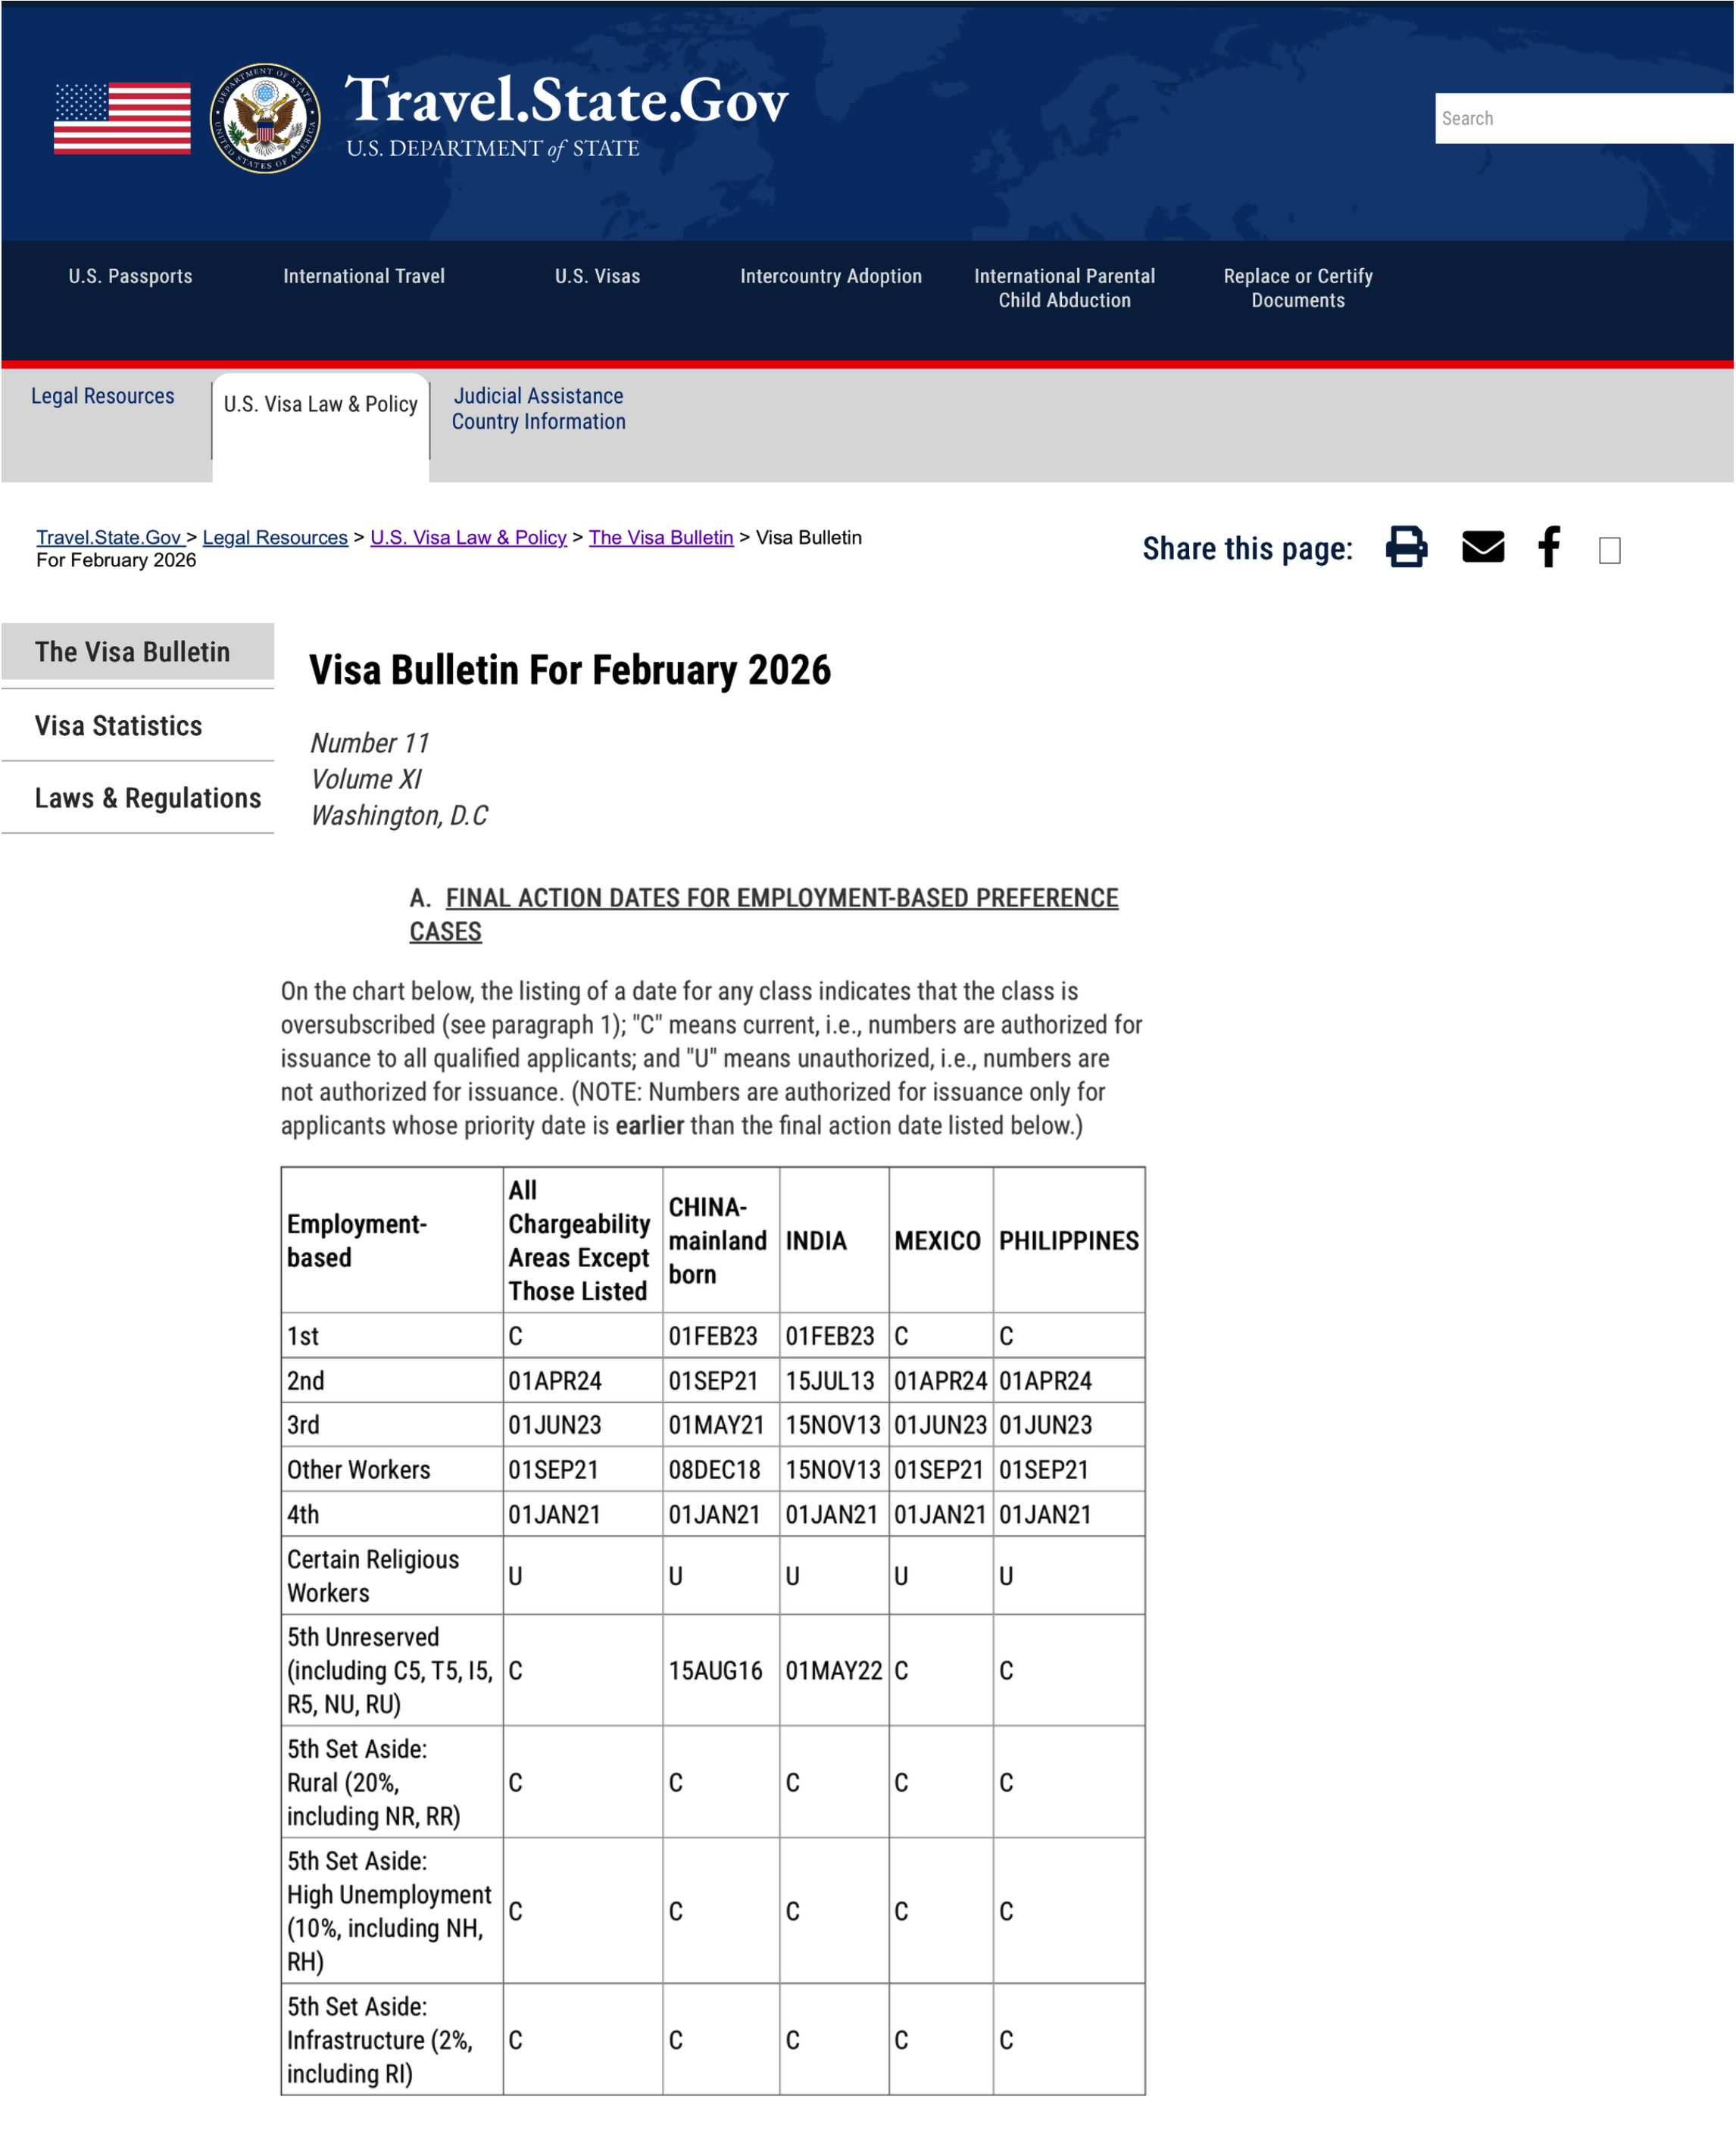
\includegraphics[width=0.50\textwidth]{visa_bulletin.png}
\caption{\footnotesize\color{uacjgray}\textit{Visa Bulletin de febrero de 2026: fechas de acción final para casos basados en empleo. Fuente: U.S. Department of State.}}
\label{fig:visa_bulletin}
\end{figure}

La administración Trump 2.0, inaugurada en enero de 2025, ha intensificado las restricciones migratorias: endurecimiento de requisitos para visas H-1B, reducción de procesamiento de ajustes de estatus, propuestas para eliminar categorías completas de inmigración familiar, y una retórica política que convierte a los inmigrantes en el enemigo. En este contexto, la pregunta que este proyecto plantea no es meramente académica; es profundamente \textbf{humana}:

\begin{notebox}
\textbf{¿Puede la inteligencia artificial encontrar asignaciones de visas que sean simultáneamente eficientes, equitativas y que minimicen el sufrimiento humano causado por décadas de espera?}
\end{notebox}

Este proyecto propone abordar la asignación de Green Cards como un \textbf{problema de optimización multiobjetivo combinatorio}, utilizando una metaheurística bio-inspirada moderna, la \textbf{Optimización por Halcones de Harris (Harris Hawks Optimization, HHO)}, para explorar el frente de Pareto de soluciones que equilibren tiempos de espera, equidad entre nacionalidades y utilización máxima de visas disponibles.

No es un ejercicio abstracto. Es un problema que los autores de este trabajo \textbf{viven en carne propia}.

% ==========================================================
% SECCION 2. SELECCIÓN DE LA METAHEURÍSTICA
% ==========================================================
\section{Selección y Originalidad de la Metaheurística}

\subsection{Algoritmos no elegibles según la carta descriptiva}

Conforme al temario de la materia \textit{Optimización Inteligente} (MIAAD, UACJ), los siguientes algoritmos serán cubiertos en clase y, por tanto, \textbf{no son elegibles} para este proyecto:

\begin{table}[H]
\centering
\caption{Metaheurísticas cubiertas en el programa del curso.}
\label{tab:prohibidos}
\renewcommand{\arraystretch}{1.3}
\begin{tabular}{clc}
\toprule
\rowcolor{tablehead}
\textcolor{white}{\textbf{Unidad}} & \textcolor{white}{\textbf{Metaheurística / Familia}} & \textcolor{white}{\textbf{Estatus}} \\
\midrule
2 & Algoritmos Genéticos (GA) & \textcolor{alertred}{\ding{55}} \\
\rowcolor{gray!8}
3 & Optimización por Enjambre de Partículas (PSO) & \textcolor{alertred}{\ding{55}} \\
3 & Colonias de Hormigas (ACO) & \textcolor{alertred}{\ding{55}} \\
\rowcolor{gray!8}
3 & Colonias de Abejas Artificiales (ABC) & \textcolor{alertred}{\ding{55}} \\
4 & Estrategias Evolutivas (ES) & \textcolor{alertred}{\ding{55}} \\
\rowcolor{gray!8}
4 & Programación Evolutiva (EP) & \textcolor{alertred}{\ding{55}} \\
5 & Búsqueda Tabú & \textcolor{alertred}{\ding{55}} \\
\rowcolor{gray!8}
5 & Recocido Simulado (SA) & \textcolor{alertred}{\ding{55}} \\
6 & NSGA-II / MOEA/D (multiobjetivo con GA) & \textcolor{alertred}{\ding{55}} \\
\bottomrule
\end{tabular}
\end{table}

\subsection{Algoritmo seleccionado: Harris Hawks Optimization (HHO)}

Se propone la \textbf{Optimización por Halcones de Harris (Harris Hawks Optimization, HHO)}, publicada por \textcite{heidari2019} en la revista \textit{Future Generation Computer Systems} (Q1, Elsevier). HHO acumula más de \textbf{5,000 citaciones} según Google Scholar, posicionándose como una de las metaheurísticas más influyentes de la última década.

\begin{resultbox}
\textbf{Referencia original:}\\[4pt]
\fullcite{heidari2019}
\end{resultbox}

\subsection{Justificación de la selección}

La elección de HHO se sustenta en cinco argumentos:

\textbf{(1) Originalidad y elegibilidad.} HHO no pertenece a ninguna de las familias cubiertas en el temario. No es un algoritmo genético, no es de enjambre de partículas, no es de colonias de hormigas ni de abejas, no es una estrategia evolutiva, y no es búsqueda tabú ni recocido simulado. Es una metaheurística basada en el comportamiento de caza cooperativa de los halcones de Harris: una inspiración biológica distinta a todas las anteriores.

\textbf{(2) Modernidad.} Publicado en 2019, cumple con el requisito de ser reciente (menor a 7 años). Además, múltiples extensiones se han publicado entre 2020 y 2025 \parencite{kusoglu2020, cerci2022, zhang2023}.

\textbf{(3) Extensión multiobjetivo demostrada.} Existen variantes MOHHO (Multi-Objective Harris Hawks Optimizer) validadas contra NSGA-II, MOPSO y otros algoritmos multiobjetivo establecidos \parencite{kusoglu2020, cerci2022, liwu2023}.

\textbf{(4) Riqueza operacional.} HHO emplea \textbf{seis operadores distintos} (dos de exploración y cuatro de explotación) gobernados por un mecanismo de energía de escape que selecciona dinámicamente la estrategia apropiada en cada iteración. Esta riqueza operacional lo distingue de otras metaheurísticas modernas. Por ejemplo, el algoritmo \textbf{JAYA} (palabra sánscrita que significa <<victoria>>), propuesto por Rao en 2016, opera con únicamente \textbf{2 operadores}: uno que acerca las soluciones hacia la mejor encontrada y otro que las aleja de la peor, sin requerir parámetros específicos pero con capacidad limitada de diversificación. Por su parte, \textbf{GWO} (\textit{Grey Wolf Optimizer}, Optimización por Lobos Grises), propuesto por Mirjalili en 2014, modela la jerarquía social de las manadas de lobos grises ($\alpha$, $\beta$, $\delta$, $\omega$) y emplea \textbf{3 operadores}: cerco, acoso y ataque de la presa. Aunque GWO ha demostrado buen rendimiento en problemas continuos, su menor número de estrategias limita su capacidad para navegar paisajes de optimización con restricciones discontinuas. Los seis operadores de HHO, en contraste, permiten transiciones fluidas entre búsqueda global amplia y refinamiento local intensivo, con los vuelos de Lévy proporcionando un mecanismo adicional de escape de óptimos locales del que carecen tanto JAYA como GWO.

\textbf{(5) Mínimos parámetros de ajuste.} Más allá del tamaño de población $N$ y el número máximo de iteraciones $T$, HHO no requiere parámetros adicionales, lo cual es una ventaja práctica para la implementación.

\newpage

% ==========================================================
% SECCION 3. DESCRIPCIÓN CONCEPTUAL
% ==========================================================
\section{Descripción Conceptual de la Metaheurística}

\subsection{Inspiración biológica: la cacería cooperativa}


\begin{figure}[H]
\centering
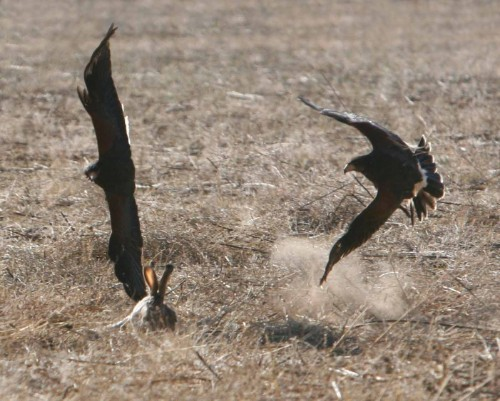
\includegraphics[width=0.48\textwidth]{harris_hawks.jpg}
\caption{\footnotesize\color{uacjgray}\textit{Halcones de Harris (Parabuteo unicinctus) en formación de caza cooperativa. Fuente: Coulson Harris's Hawks.}}
\label{fig:hawks}
\end{figure}

El halcón de Harris (\textit{Parabuteo unicinctus}) es una de las pocas aves rapaces que cazan en grupos coordinados. Su estrategia, conocida como \textbf{<<\,surprise pounce\,>>} (embestida sorpresa), consiste en que un grupo de halcones rodea a la presa (típicamente un conejo) desde múltiples direcciones y la ataca simultáneamente, adaptando su estrategia según el nivel de energía que la presa conserva para escapar \parencite{heidari2019}.

Esta metáfora se traduce al dominio de la optimización:

\begin{table}[H]
\centering
\caption{Mapeo entre la naturaleza y la optimización.}
\label{tab:mapeo}
\renewcommand{\arraystretch}{1.3}
\begin{tabular}{ll}
\toprule
\rowcolor{tablehead}
\textcolor{white}{\textbf{Elemento biológico}} & \textcolor{white}{\textbf{Equivalente en optimización}} \\
\midrule
Halcón individual & Solución candidata en la población \\
\rowcolor{gray!8}
Presa (conejo) & Mejor solución encontrada (o líder Pareto) \\
Energía de escape de la presa & Parámetro $E$ que controla exploración/explotación \\
\rowcolor{gray!8}
Estrategias de caza & Operadores de movimiento (6 distintos) \\
Posición del halcón & Vector de decisión $\mathbf{X}_i$ \\
\rowcolor{gray!8}
Éxito de captura & Valor de la función objetivo (fitness) \\
\bottomrule
\end{tabular}
\end{table}

\subsection{Mecanismo de exploración vs. explotación}

El balance entre exploración (búsqueda global) y explotación (búsqueda local) se gobierna mediante la \textbf{energía de escape} $E$:

\begin{formulabox}
\begin{equation}
E = 2E_0 \left(1 - \frac{t}{T}\right)
\label{eq:energy}
\end{equation}
\end{formulabox}

donde $E_0 \in [-1, 1]$ es un valor aleatorio que se regenera en cada iteración, $t$ es la iteración actual y $T$ es el número máximo de iteraciones.

La lógica de transición es:

\begin{itemize}
    \item \textbf{$|E| \geq 1$:} La presa tiene alta energía de escape $\Rightarrow$ los halcones \textbf{exploran} ampliamente el espacio de búsqueda (búsqueda global).
    \item \textbf{$|E| < 1$:} La presa está agotada $\Rightarrow$ los halcones \textbf{explotan} regiones prometedoras (búsqueda local refinada).
\end{itemize}

Dado que $E_0$ es estocástico, HHO \textbf{no sigue un esquema rígido} de transición. El algoritmo oscila entre exploración y explotación a lo largo de toda la ejecución, con la explotación dominando progresivamente. Esta propiedad es crítica para evitar la convergencia prematura \parencite{heidari2019, alabool2021}.

\begin{figure}[H]
\centering
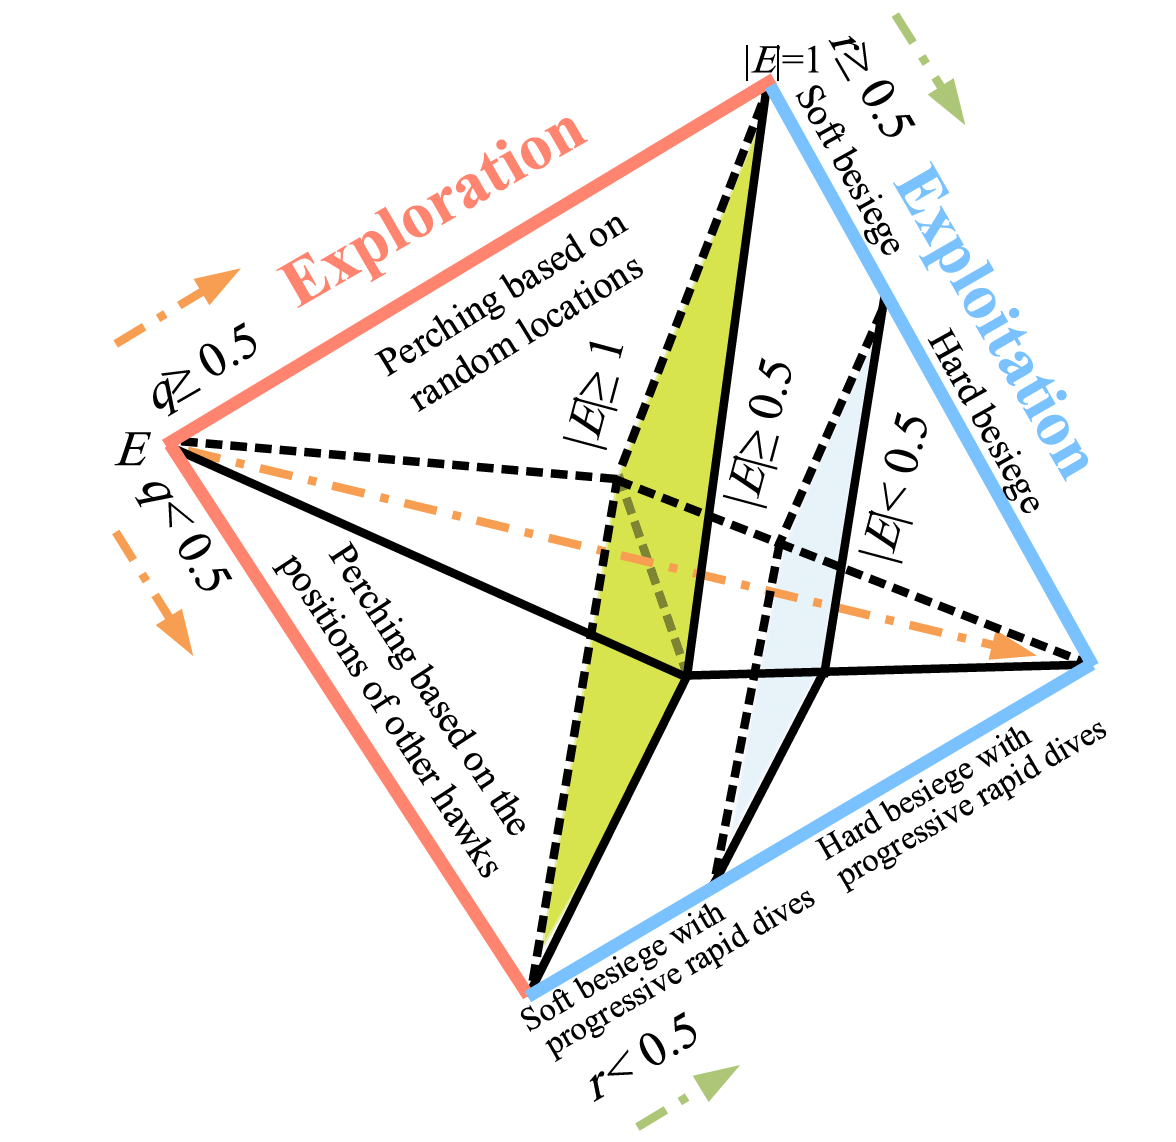
\includegraphics[width=0.60\textwidth]{hho_fases.png}
\caption{\footnotesize\color{uacjgray}\textit{Fases de exploración y explotación del algoritmo HHO, mostrando la selección de operadores según los parámetros E, q y r. Fuente: Heidari et al. (2019).}}
\label{fig:fases_hho}
\end{figure}

% ==========================================================
% SECCION 4: DIAGRAMA GENERAL DEL ALGORITMO HHO
% ==========================================================

\section{Diagrama General del Algoritmo HHO}

El siguiente diagrama presenta de forma visual y simplificada las cinco fases fundamentales del algoritmo Harris Hawks Optimization (HHO), desde la dispersión inicial de la población hasta la convergencia hacia la solución óptima. La analogía entre la cacería cooperativa de los halcones de Harris y el proceso de optimización se ilustra paso a paso, facilitando la comprensión del mecanismo adaptativo que gobierna la transición entre exploración y explotación.


\begin{figure}[H]
\centering
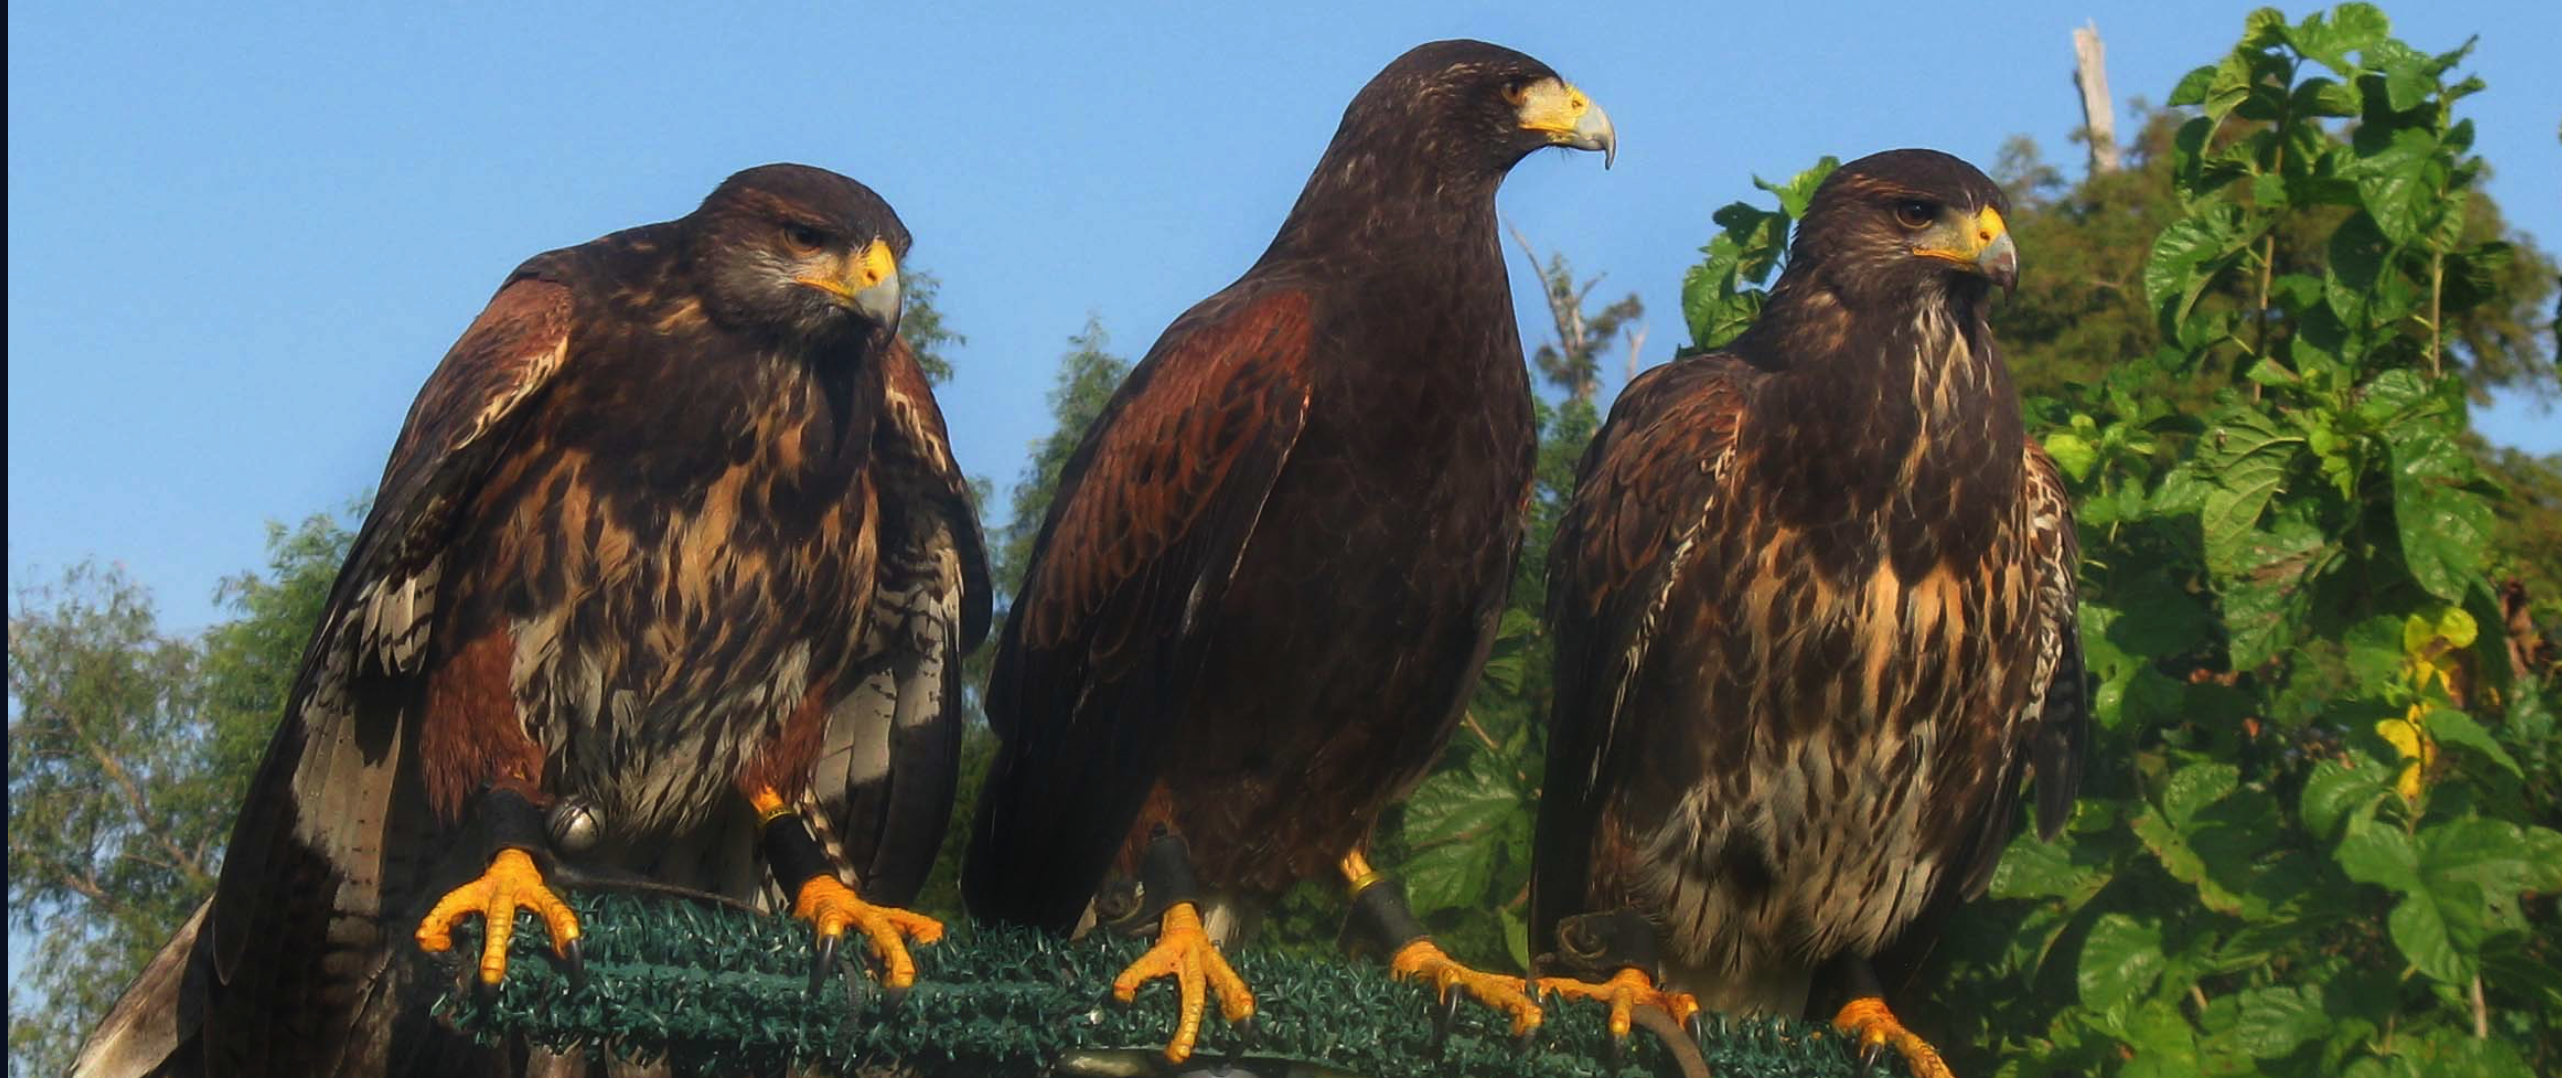
\includegraphics[width=0.85\textwidth]{harris_hawks_trio.png}
\caption{\footnotesize\color{uacjgray}\textit{Trío de halcones de Harris (Parabuteo unicinctus). Fuente: Coulson Harris's Hawks.}}
\label{fig:hawks_trio}
\end{figure}

\newpage

\begin{figure}[H]
\centering
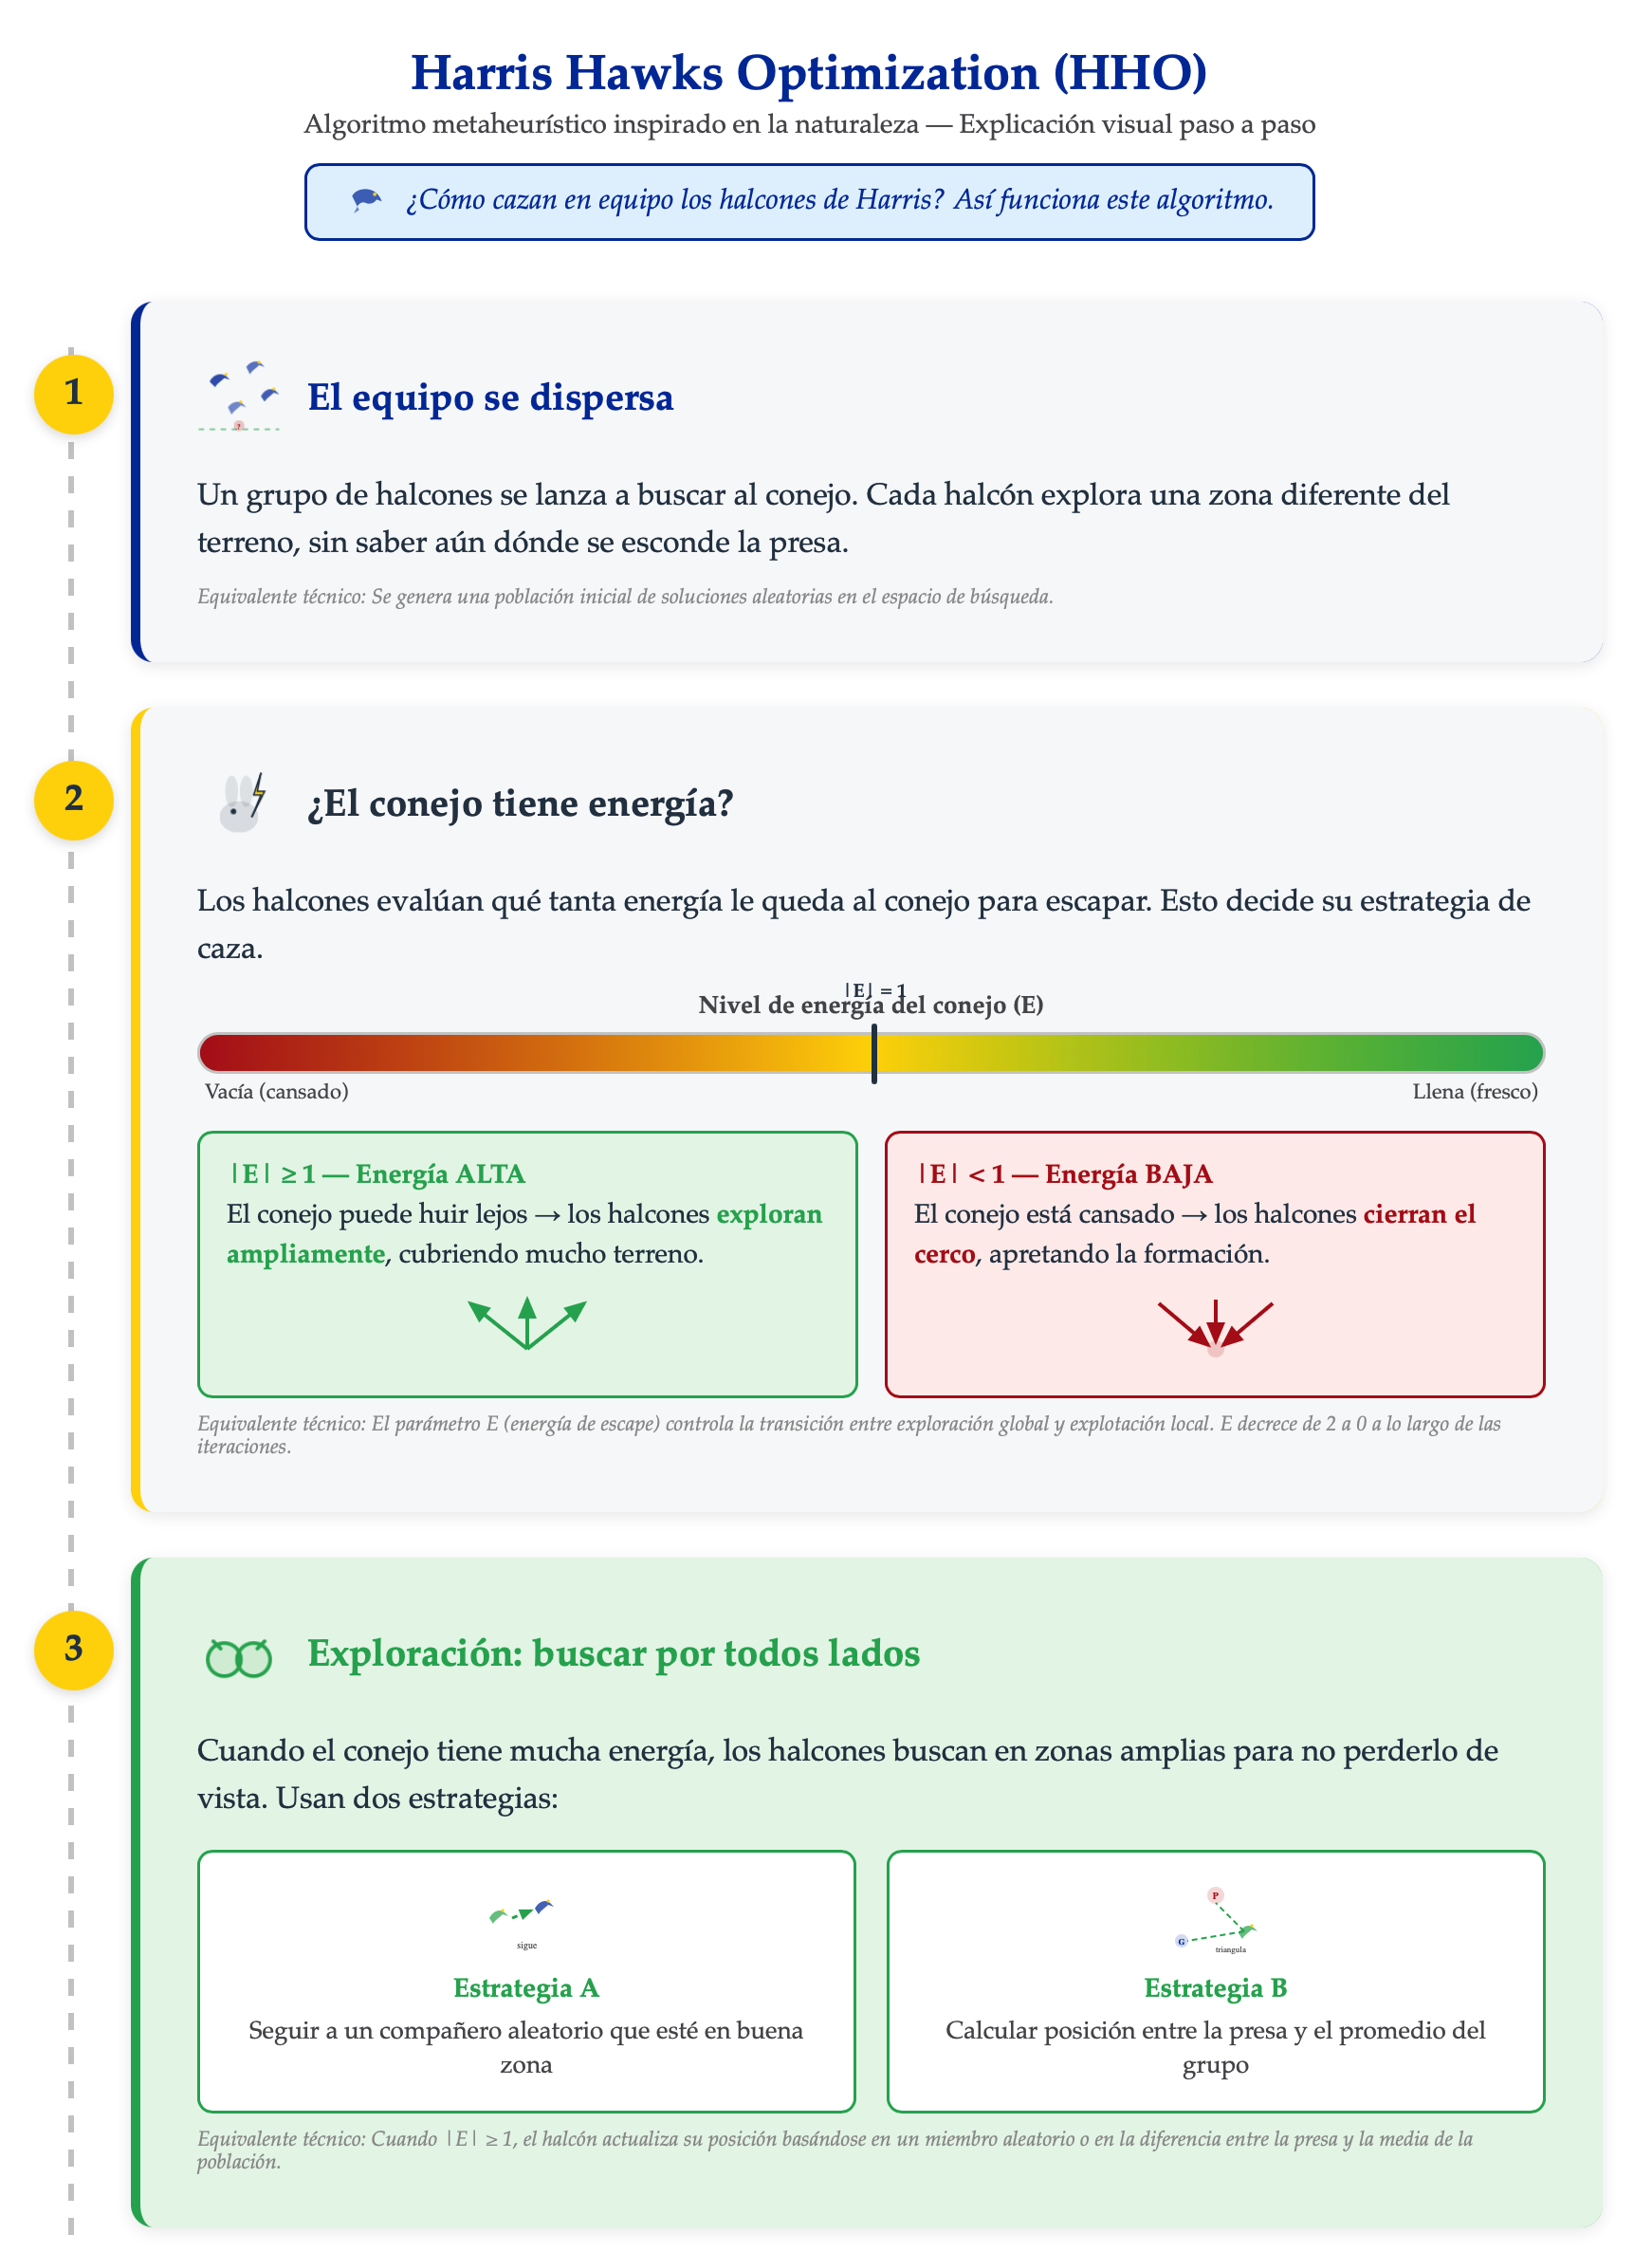
\includegraphics[width=\textwidth, height=1.1\textheight, keepaspectratio]{Diagrama_General_p1.png}
\caption{\footnotesize\color{uacjgray}\textit{Diagrama general del algoritmo HHO, parte 1: inicialización, evaluación de energía y fase de exploración. Elaboración propia.}}
\label{fig:diagrama_p1}
\end{figure}

\newpage

\begin{figure}[H]
\centering
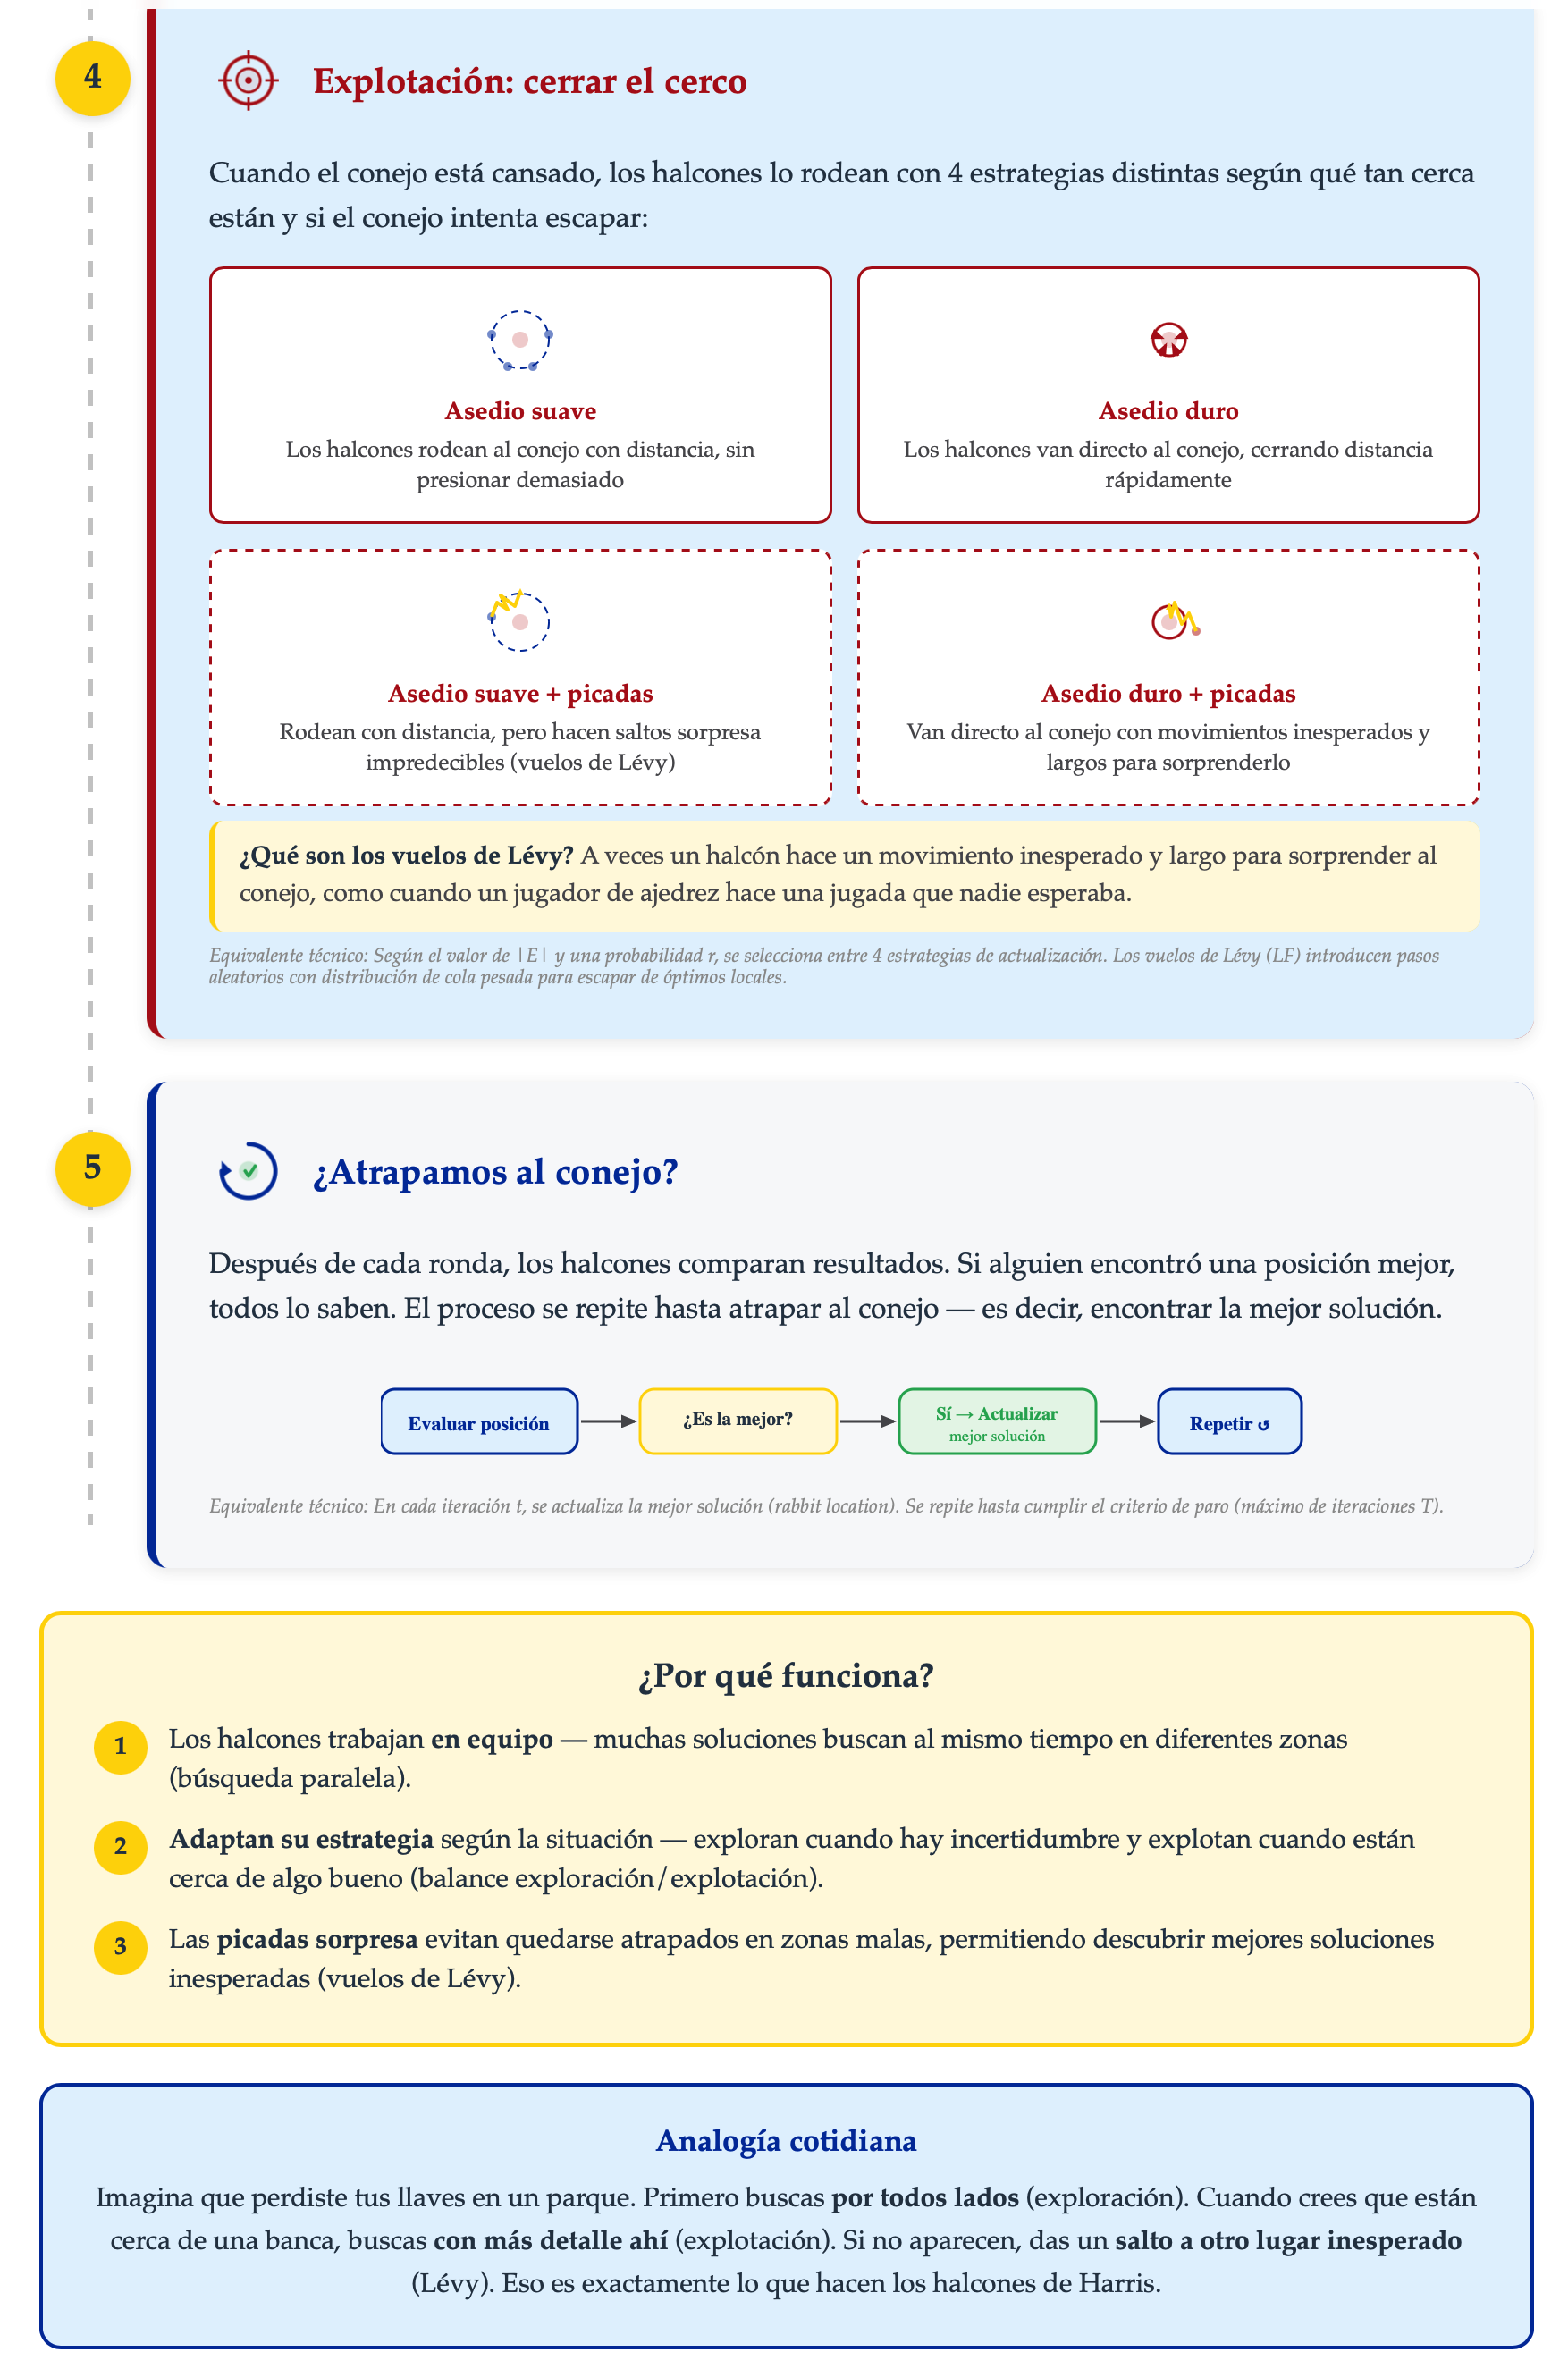
\includegraphics[width=\textwidth, height=0.99\textheight, keepaspectratio]{Diagrama_General_p2.png}
\caption{\footnotesize\color{uacjgray}\textit{Diagrama general del algoritmo HHO, parte 2: fase de explotación, vuelos de Lévy y convergencia. Elaboración propia.}}
\label{fig:diagrama_p2}
\end{figure}



% ==========================================================
% 5. DEFINICIÓN DE OPERADORES
% ==========================================================
\section{Definición y Explicación de Operadores}

HHO emplea \textbf{seis operadores} organizados en dos fases: exploración (2 operadores) y explotación (4 operadores). La selección del operador se realiza dinámicamente en función de la energía $E$ y dos parámetros aleatorios $q$ y $r$ \parencite{heidari2019}.

\subsection{Operador 0: Inicialización}

Se genera una población de $N$ halcones uniformemente distribuidos dentro de los límites del espacio de búsqueda $[LB, UB]$:

\begin{formulabox}
\begin{equation}
X_i^{(0)} = LB + \text{rand} \times (UB - LB), \quad i = 1, \ldots, N
\label{eq:init}
\end{equation}
\end{formulabox}

Se evalúa el fitness de cada halcón y se designa al mejor como la \textbf{posición de la presa} $\mathbf{X}_{\text{rabbit}}$.

\subsection{Fase de exploración (\texorpdfstring{$|E| \geq 1$}{|E|>=1})}

Cuando la presa conserva alta energía, los halcones buscan ampliamente. Un parámetro aleatorio $q \in [0,1]$ selecciona entre dos estrategias equiprobables:

\subsubsection{Operador 1: Perchado aleatorio (\texorpdfstring{$q \geq 0.5$}{q>=0.5})}

\begin{formulabox}
\begin{equation}
\mathbf{X}_i(t+1) = \mathbf{X}_{\text{rand}}(t) - r_1 \left| \mathbf{X}_{\text{rand}}(t) - 2r_2 \, \mathbf{X}_i(t) \right|
\label{eq:explor1}
\end{equation}
\end{formulabox}

donde $\mathbf{X}_{\text{rand}}$ es un halcón seleccionado aleatoriamente y $r_1, r_2 \in [0,1]$ son números aleatorios.

\subsubsection{Operador 2: Perchado presa-media (\texorpdfstring{$q < 0.5$}{q<0.5})}

\begin{formulabox}
\begin{equation}
\mathbf{X}_i(t+1) = \left(\mathbf{X}_{\text{rabbit}}(t) - \mathbf{X}_m(t)\right) - r_3\left(LB + r_4(UB - LB)\right)
\label{eq:explor2}
\end{equation}
\end{formulabox}

donde $\mathbf{X}_m(t) = \frac{1}{N}\sum_{i=1}^{N} \mathbf{X}_i(t)$ es la posición media y $r_3, r_4 \in [0,1]$ son aleatorios.

\subsection{Fase de explotación (\texorpdfstring{$|E| < 1$}{|E|<1}): las cuatro estrategias de embestida}

Se definen el vector de diferencia $\Delta \mathbf{X}(t) = \mathbf{X}_{\text{rabbit}}(t) - \mathbf{X}_i(t)$ y la fuerza de salto $J = 2(1 - r_5)$, con $r_5 \in [0,1]$. Un segundo parámetro $r \in [0,1]$ modela la probabilidad de escape de la presa.

\subsubsection{Operador 3: Asedio suave (\texorpdfstring{$r \geq 0.5$, $|E| \geq 0.5$}{r>=0.5, |E|>=0.5})}

La presa conserva energía para escapar. Los halcones la rodean con movimientos suaves:

\begin{formulabox}
\begin{equation}
\mathbf{X}_i(t+1) = \Delta \mathbf{X}(t) - E \left| J \cdot \mathbf{X}_{\text{rabbit}}(t) - \mathbf{X}_i(t) \right|
\label{eq:soft_besiege}
\end{equation}
\end{formulabox}

\subsubsection{Operador 4: Asedio duro (\texorpdfstring{$r \geq 0.5$, $|E| < 0.5$}{r>=0.5, |E|<0.5})}

La presa está exhausta. Los halcones cierran agresivamente:

\begin{formulabox}
\begin{equation}
\mathbf{X}_i(t+1) = \mathbf{X}_{\text{rabbit}}(t) - E \left| \Delta \mathbf{X}(t) \right|
\label{eq:hard_besiege}
\end{equation}
\end{formulabox}

\subsubsection{Operador 5: Asedio suave con Lévy (\texorpdfstring{$r < 0.5$, $|E| \geq 0.5$}{r<0.5, |E|>=0.5})}

La presa escapa del cerco inicial. Los halcones ejecutan patrones de inmersión basados en \textbf{vuelos de Lévy}:

\begin{formulabox}
\begin{align}
\mathbf{Y} &= \mathbf{X}_{\text{rabbit}}(t) - E \left| J \cdot \mathbf{X}_{\text{rabbit}}(t) - \mathbf{X}_i(t) \right| \label{eq:soft_levy_Y}\\[6pt]
\mathbf{Z} &= \mathbf{Y} + \mathbf{S} \times LF(D) \label{eq:soft_levy_Z}
\end{align}
\end{formulabox}

donde $\mathbf{S}$ es un vector aleatorio de dimensión $D$ y $LF$ es la función de vuelo de Lévy:

\begin{formulabox}
\begin{equation}
LF(x) = 0.01 \times \frac{u \cdot \sigma}{|v|^{1/\beta}}, \;\;
\sigma = \!\left[\frac{\Gamma(1\!+\!\beta)\sin(\pi\beta/2)}{\Gamma\!\bigl(\frac{1+\beta}{2}\bigr)\,\beta \cdot 2^{(\beta-1)/2}}\right]^{\!1/\beta}
\label{eq:levy}
\end{equation}
\end{formulabox}

con $u, v \sim \mathcal{N}(0,1)$ y $\beta = 1.5$. Se emplea \textbf{selección greedy}: el halcón adopta $\mathbf{Y}$ si mejora su fitness; de lo contrario prueba $\mathbf{Z}$; si ninguno mejora, conserva su posición actual.

\subsubsection{Operador 6: Asedio duro con Lévy (\texorpdfstring{$r < 0.5$, $|E| < 0.5$}{r<0.5, |E|<0.5})}

Estructura idéntica al Operador 5, pero utilizando la posición media del enjambre:

\begin{formulabox}
\begin{align}
\mathbf{Y} &= \mathbf{X}_{\text{rabbit}}(t) - E \left| J \cdot \mathbf{X}_{\text{rabbit}}(t) - \mathbf{X}_m(t) \right| \label{eq:hard_levy_Y}\\[6pt]
\mathbf{Z} &= \mathbf{Y} + \mathbf{S} \times LF(D) \label{eq:hard_levy_Z}
\end{align}
\end{formulabox}

Misma selección greedy que en el Operador 5.

\subsection{Resumen de la lógica de selección de operadores}

\begin{table}[H]
\centering
\caption{Mapa de selección de los seis operadores de HHO.}
\label{tab:operadores}
\renewcommand{\arraystretch}{1.3}
\begin{tabular}{llll}
\toprule
\rowcolor{tablehead}
\textcolor{white}{\textbf{Condición}} & \textcolor{white}{\textbf{Estrategia}} & \textcolor{white}{\textbf{Tipo}} & \textcolor{white}{\textbf{Op.}} \\
\midrule
$|E| \geq 1$, $q \geq 0.5$ & Perchado aleatorio & Exploración & 1 \\
\rowcolor{gray!8}
$|E| \geq 1$, $q < 0.5$ & Perchado presa-media & Exploración & 2 \\
$|E| < 1$, $r \geq 0.5$, $|E| \geq 0.5$ & Asedio suave & Explotación & 3 \\
\rowcolor{gray!8}
$|E| < 1$, $r \geq 0.5$, $|E| < 0.5$ & Asedio duro & Explotación & 4 \\
$|E| < 1$, $r < 0.5$, $|E| \geq 0.5$ & Asedio suave + Lévy & Explotación & 5 \\
\rowcolor{gray!8}
$|E| < 1$, $r < 0.5$, $|E| < 0.5$ & Asedio duro + Lévy & Explotación & 6 \\
\bottomrule
\end{tabular}
\end{table}

\begin{yellowbox}
\textbf{Nota clave:} Los vuelos de Lévy (Operadores 5 y 6) introducen saltos de largo alcance que permiten escapar de óptimos locales, una propiedad crítica para paisajes de optimización con restricciones discontinuas como los topes por país del 7\%.
\end{yellowbox}

% ==========================================================
% SECCIÓN 6: APLICACIÓN DE HHO AL PROBLEMA DE GREEN CARDS
% ==========================================================
\newpage
\section{¿Cómo los Halcones de Harris Resuelven el Problema de las Green Cards?}

El siguiente diagrama presenta el mapeo completo entre los componentes del algoritmo MOHHO y los elementos concretos del problema de asignación multiobjetivo de visas de empleo en Estados Unidos. Cada fase del algoritmo se traduce a una acción específica sobre la distribución de las 140,000 visas anuales, mostrando cómo la cacería cooperativa de los halcones se convierte en una herramienta para explorar asignaciones que equilibren tiempo de espera, equidad entre países y utilización máxima de visas.

\begin{figure}[H]
\centering
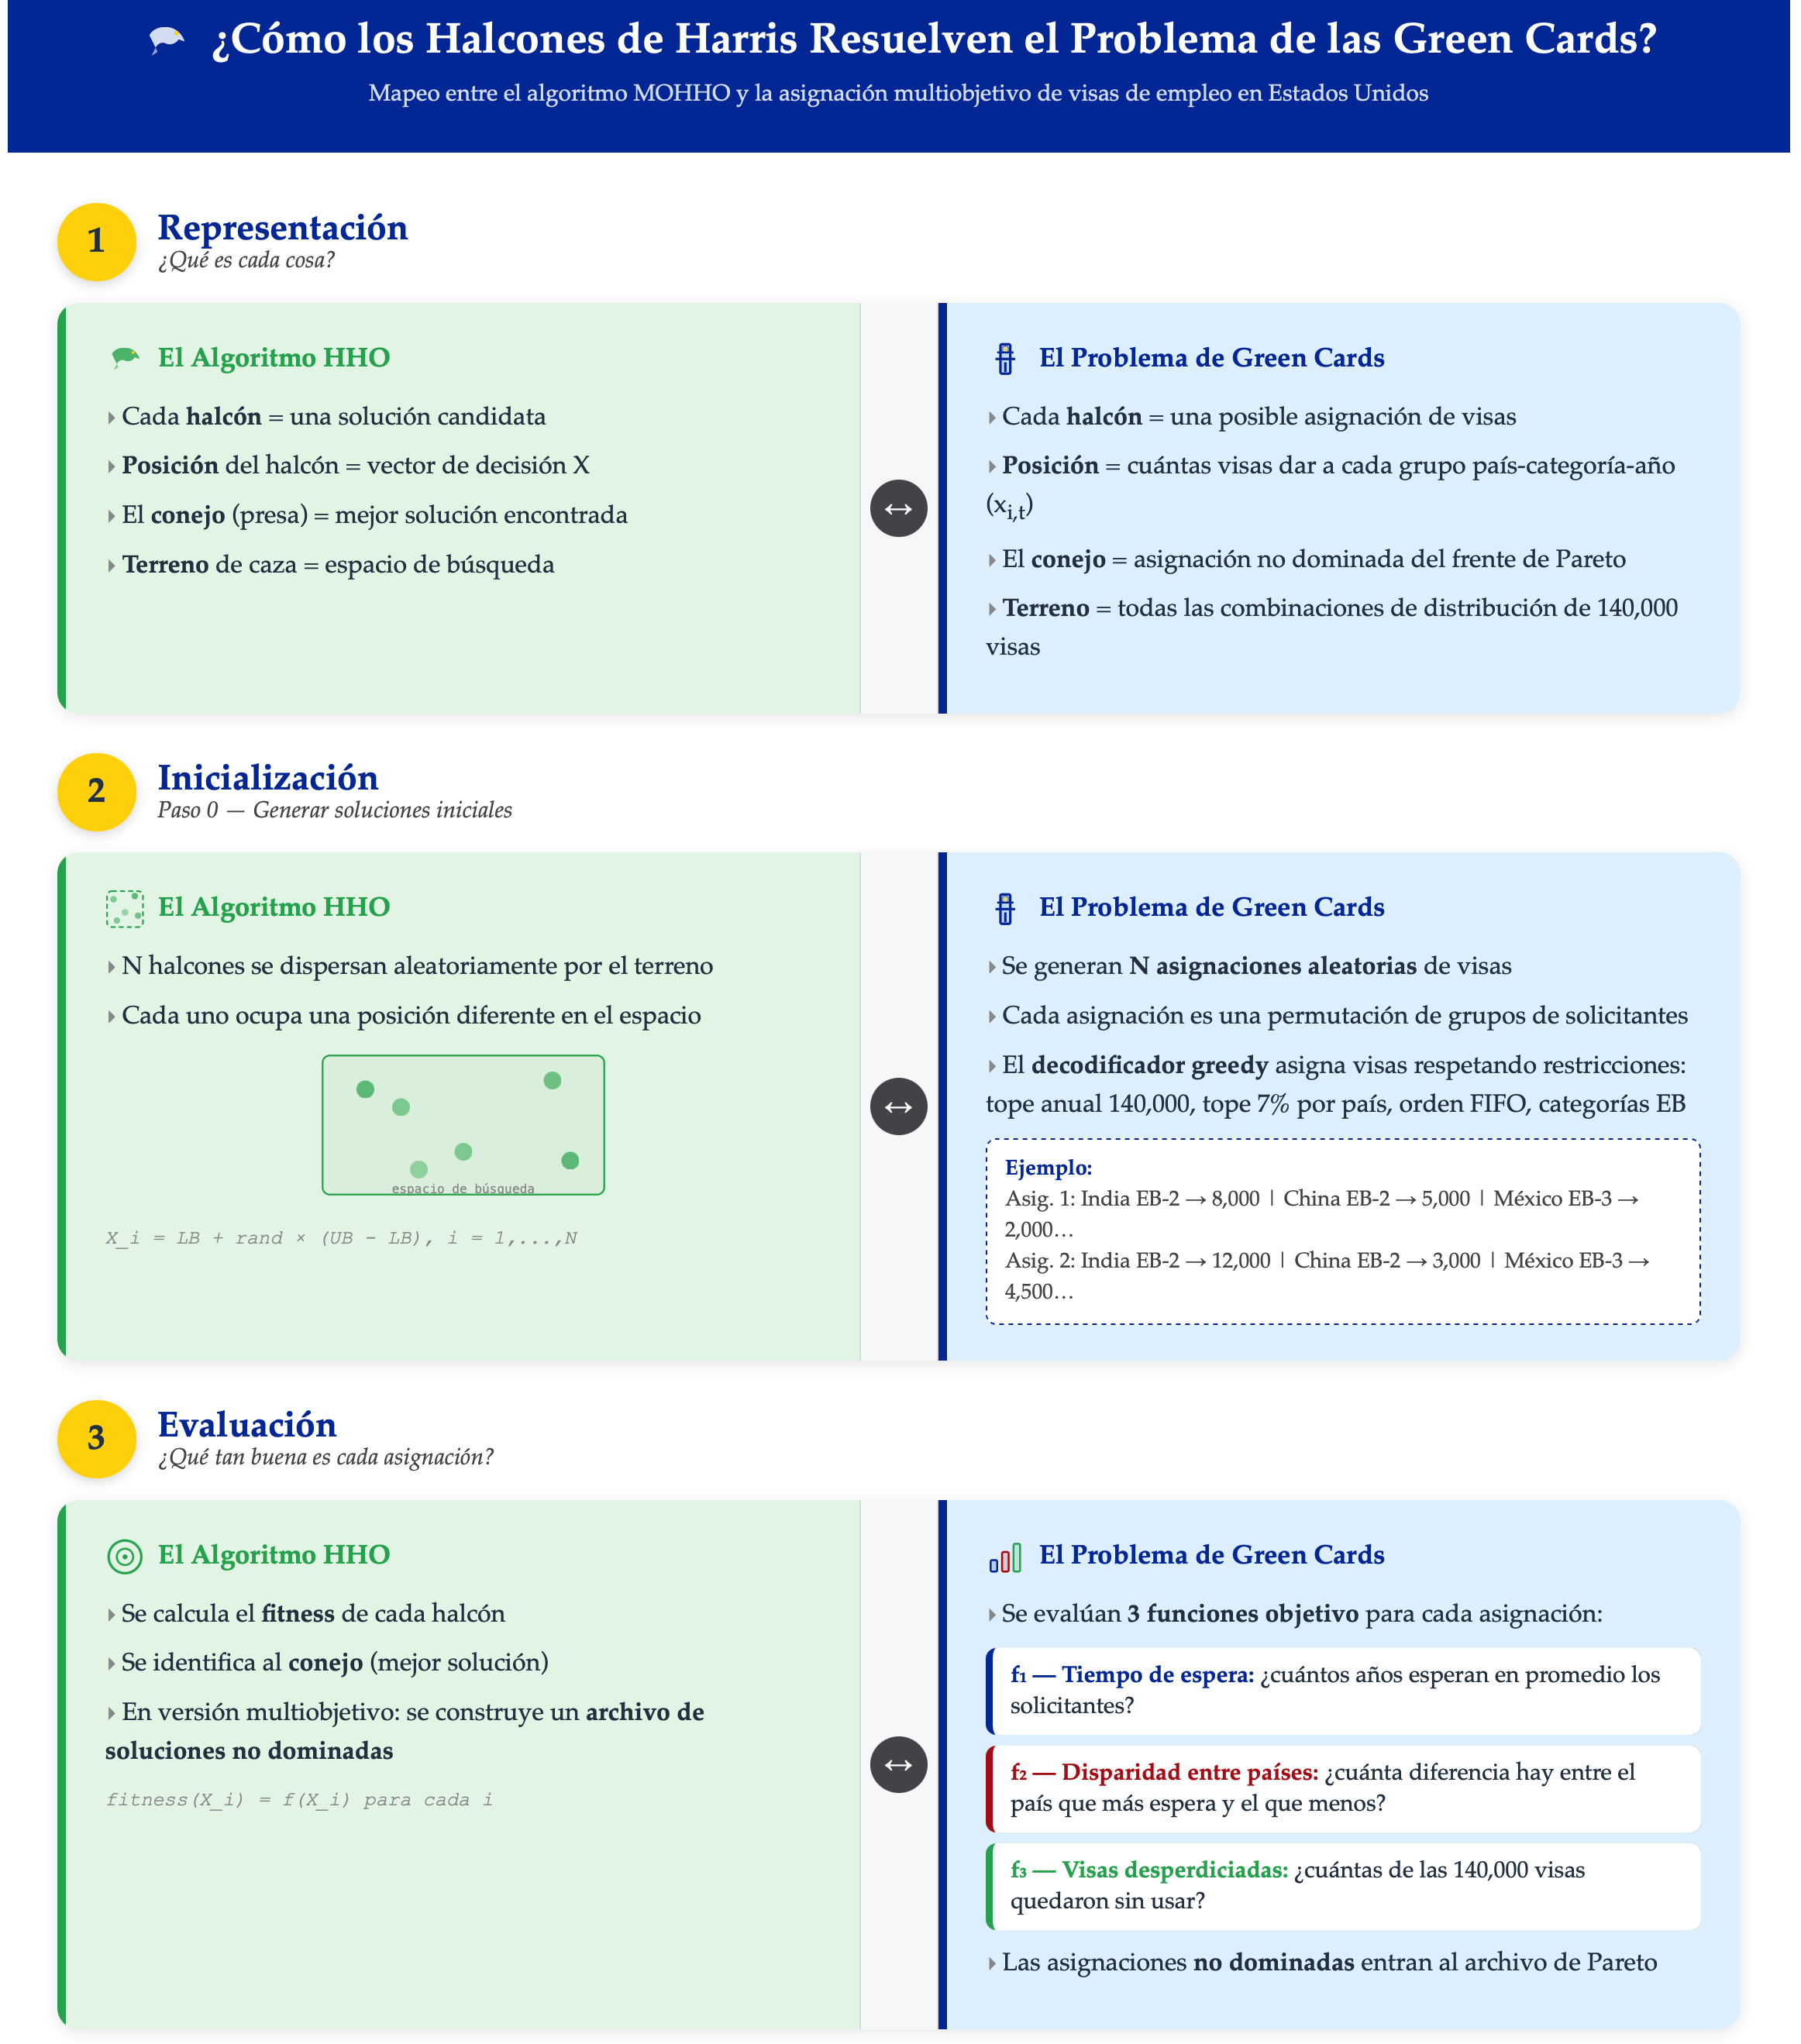
\includegraphics[width=\textwidth, height=1.60\textheight, keepaspectratio]{HalconesResuelvenp1.png}
\caption{\footnotesize\color{uacjgray}\textit{Aplicación de HHO al problema de Green Cards, parte 1: representación del problema, inicialización y evaluación de los tres objetivos. Elaboración propia.}}
\label{fig:halcones_gc_p1}
\end{figure}

\newpage

\begin{figure}[H]
\centering
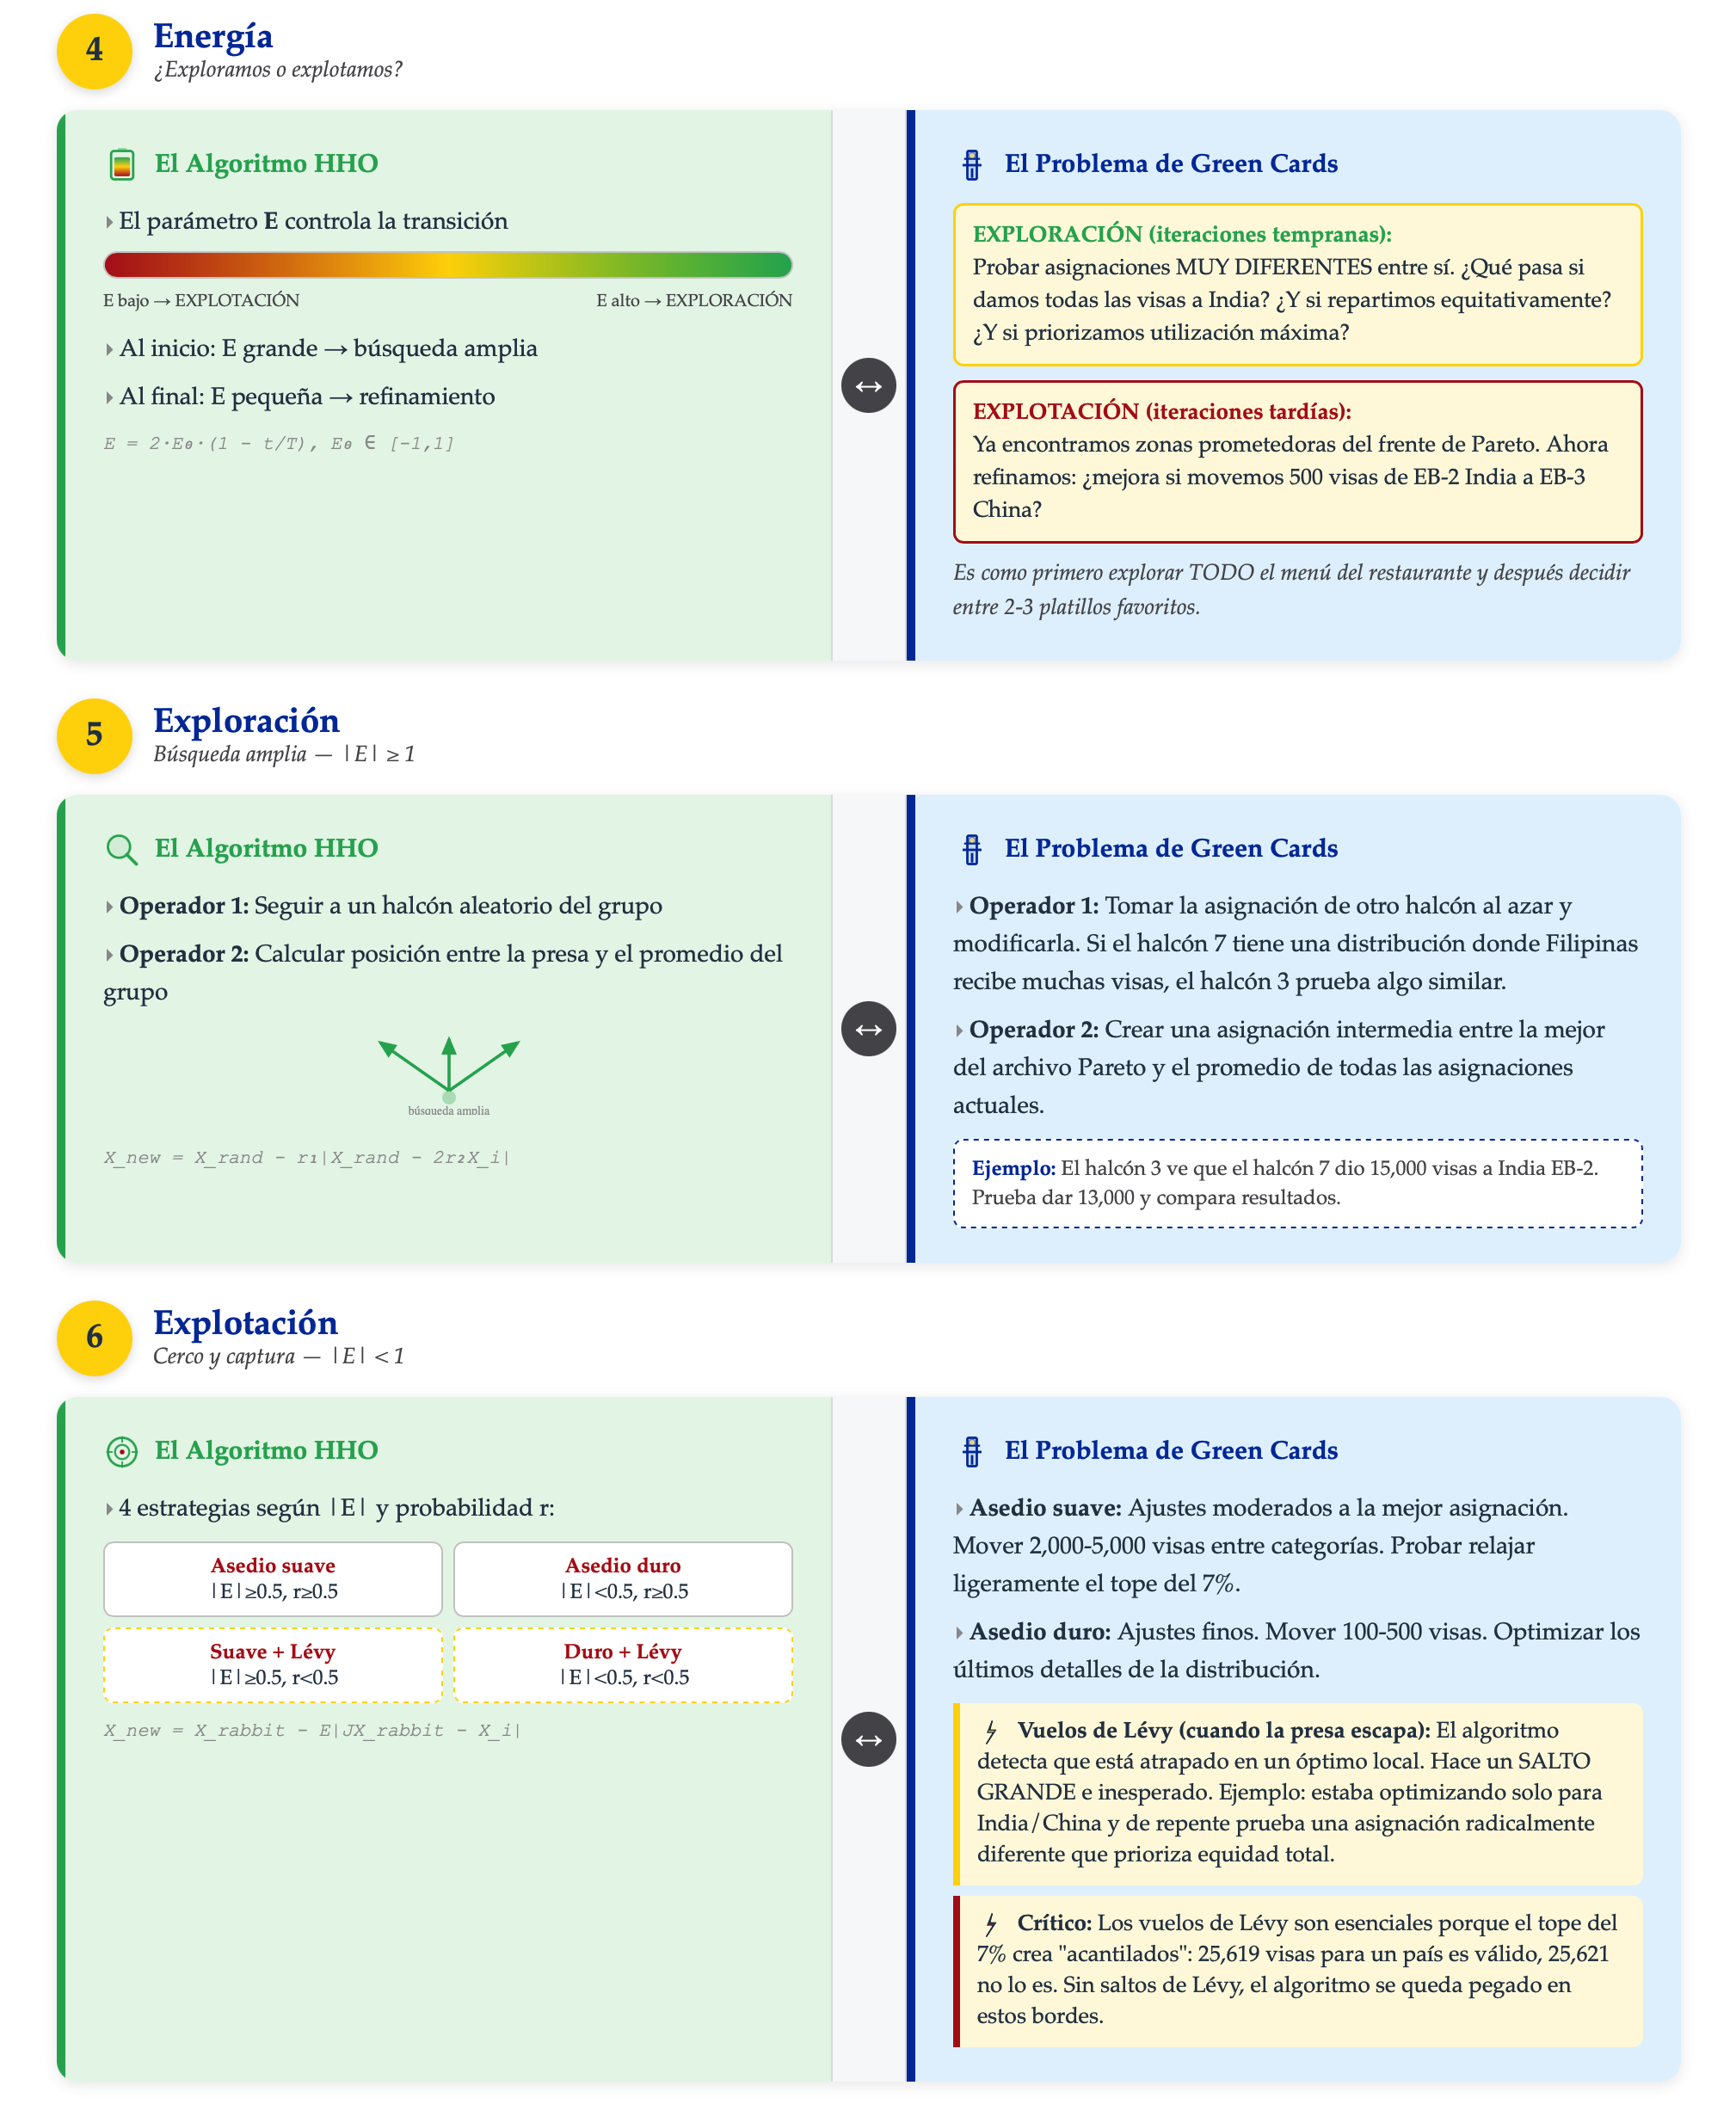
\includegraphics[width=\textwidth, height=1.60\textheight, keepaspectratio]{HalconesResuelvenp2.png}
\caption{\footnotesize\color{uacjgray}\textit{Aplicación de HHO al problema de Green Cards, parte 2: mecanismo de energía, fase de exploración y operadores de explotación. Elaboración propia.}}
\label{fig:halcones_gc_p2}
\end{figure}

\newpage

\begin{figure}[H]
\centering
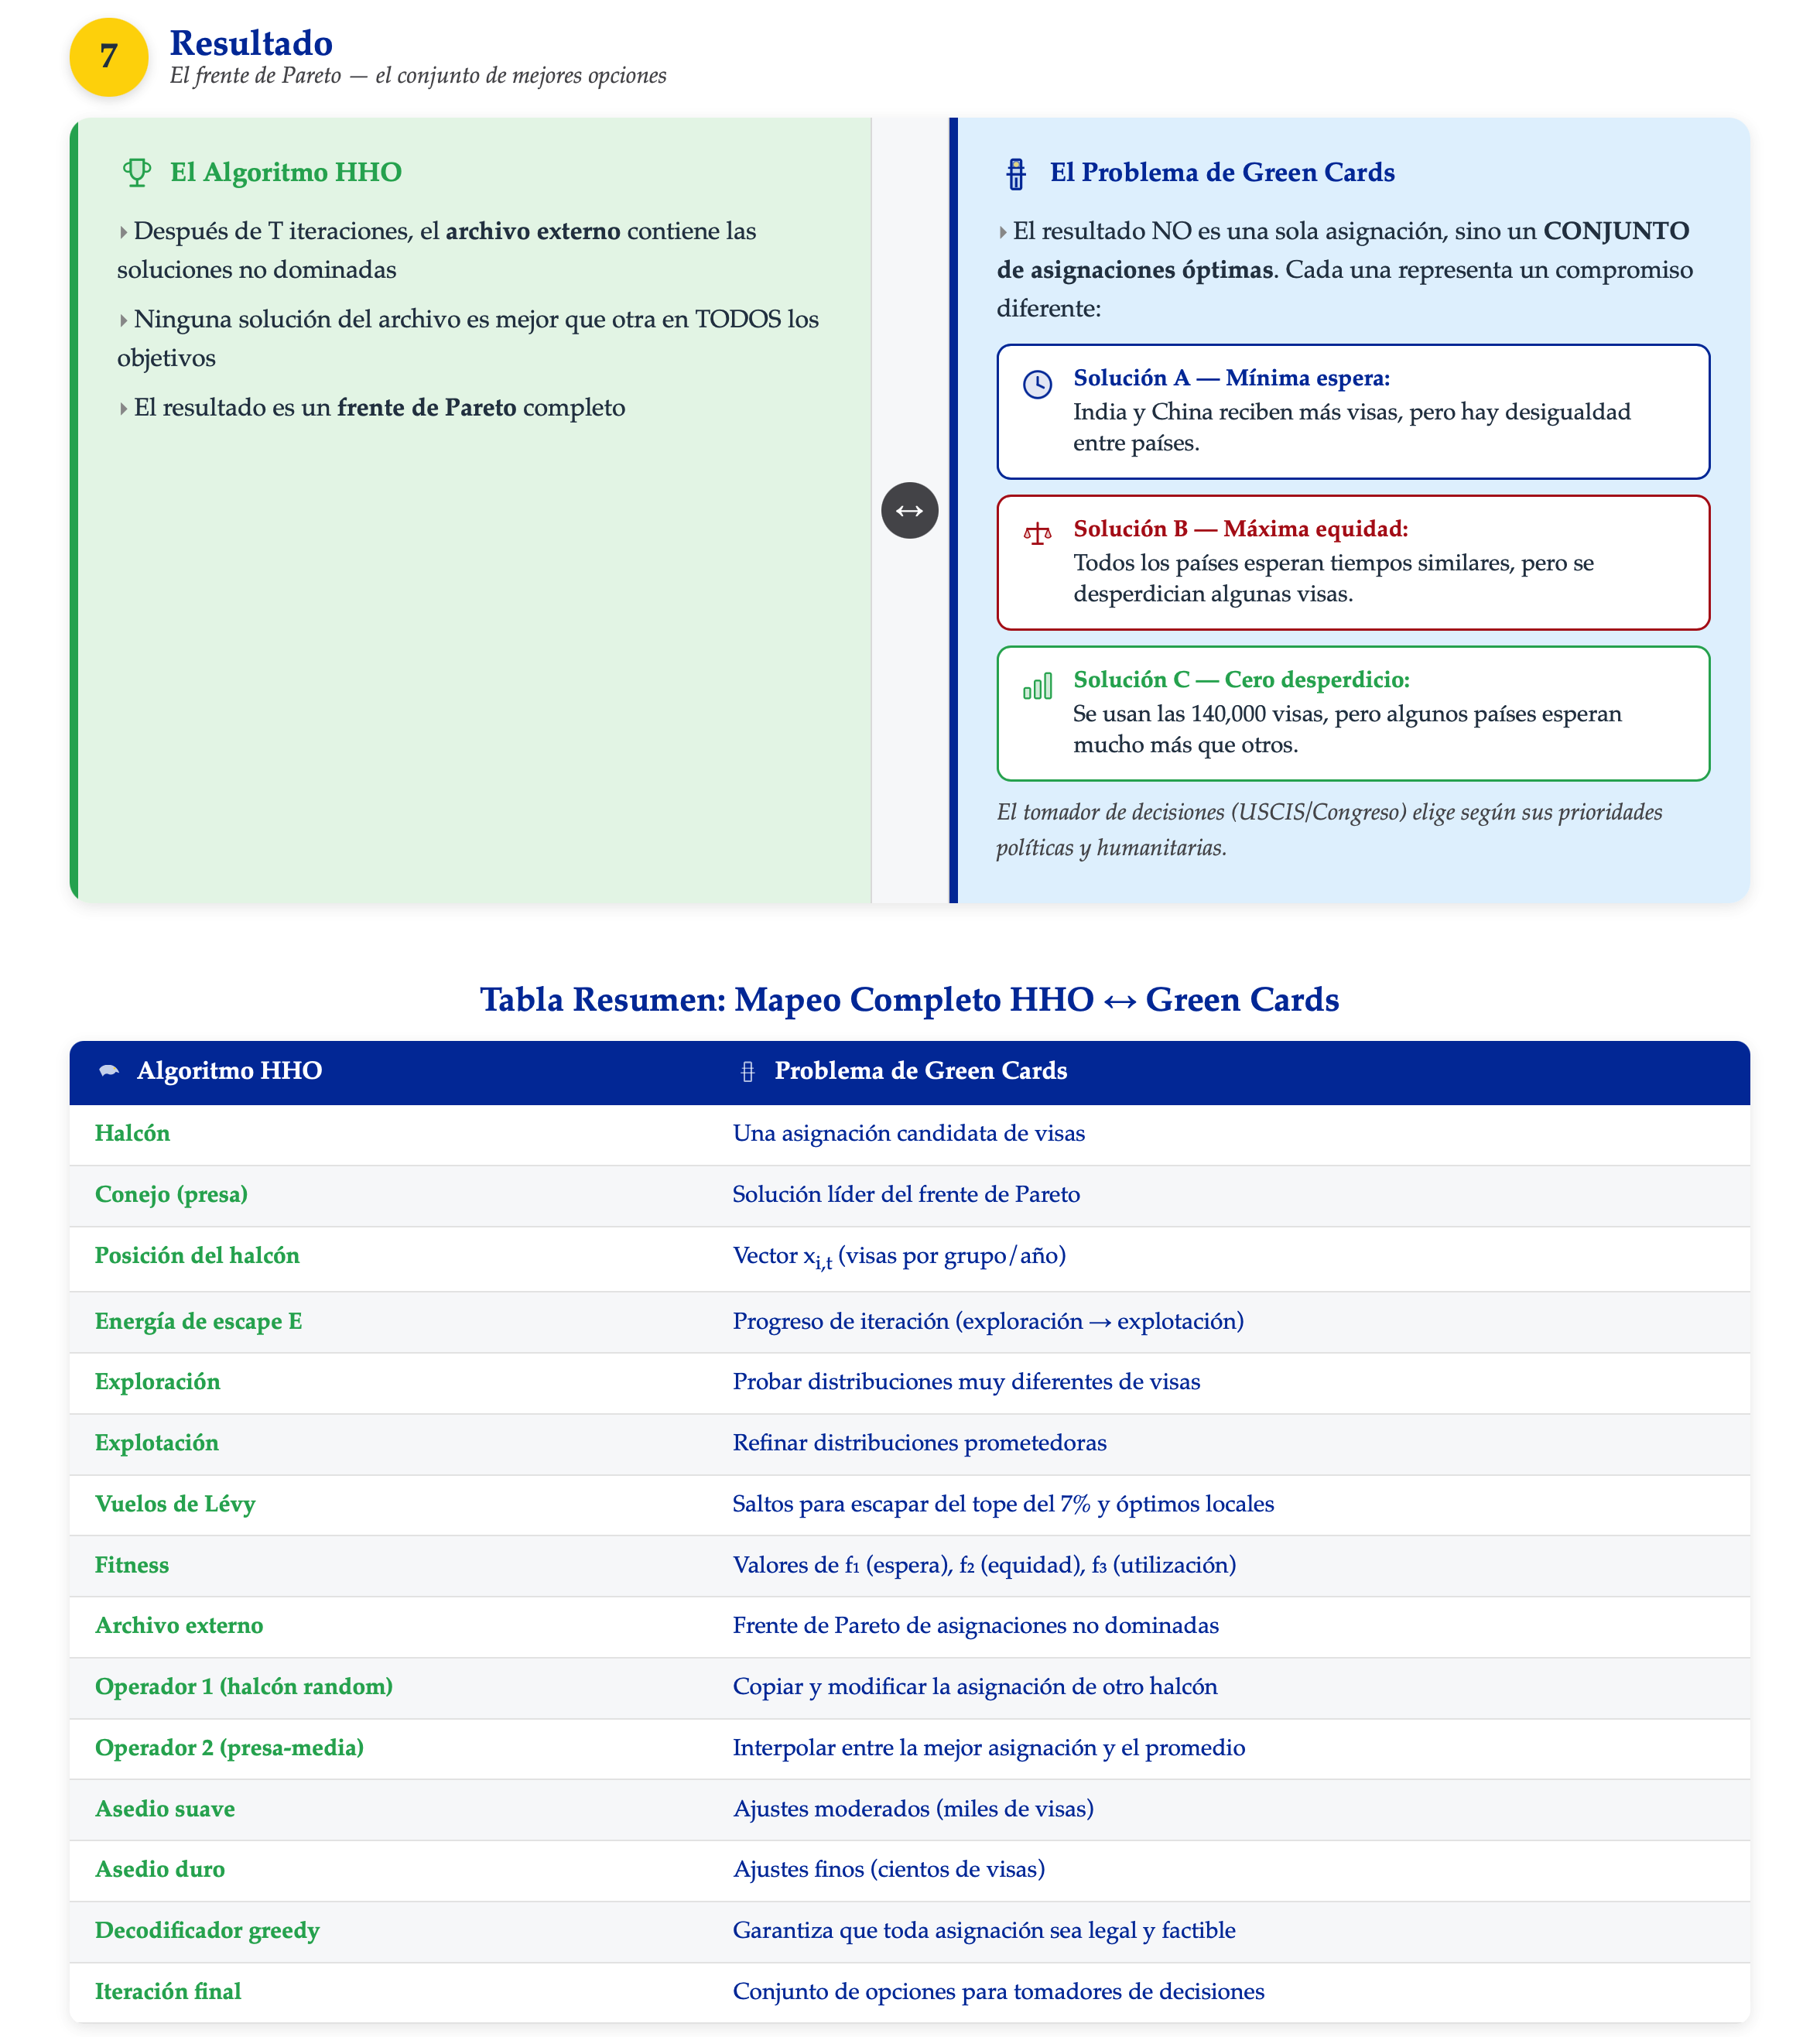
\includegraphics[width=\textwidth, height=1.60\textheight, keepaspectratio]{HalconesResuelvenp3.png}
\caption{\footnotesize\color{uacjgray}\textit{Aplicación de HHO al problema de Green Cards, parte 3: frente de Pareto resultante, tabla resumen del mapeo algoritmo-problema y soluciones ejemplo. Elaboración propia.}}
\label{fig:halcones_gc_p3}
\end{figure}


\newpage

% ==========================================================
% 7. PLANTEAMIENTO DEL PROBLEMA
% ==========================================================
\section{Planteamiento del Problema de Aplicación}

\subsection{Contexto: el sistema de Green Cards basado en empleo}

El sistema de inmigración basado en empleo de Estados Unidos asigna una base de \textbf{140,000 visas anuales} distribuidas en cinco categorías de preferencia, procesadas en orden FIFO (\textit{First-In, First-Out}) por fecha de prioridad dentro de cada combinación país-categoría. El Departamento de Estado publica mensualmente el \textit{Visa Bulletin}, que establece las fechas de corte que determinan qué solicitantes pueden avanzar \parencite{dosfeb2026}.



\begin{table}[H]
\centering
\caption{Categorías de empleo y asignación base de visas.}
\label{tab:categorias}
\renewcommand{\arraystretch}{1.3}
\begin{tabular}{clcc}
\toprule
\rowcolor{tablehead}
\textcolor{white}{\textbf{Cat.}} & \textcolor{white}{\textbf{Descripción}} & \textcolor{white}{\textbf{Porcentaje}} & \textcolor{white}{\textbf{Aprox. visas}} \\
\midrule
EB-1 & Trabajadores prioritarios & 28.6\% & $\sim$40,040 \\
\rowcolor{gray!8}
EB-2 & Profesionistas con grado avanzado & 28.6\% & $\sim$40,040 \\
EB-3 & Trabajadores calificados & 28.6\% & $\sim$40,040 \\
\rowcolor{gray!8}
EB-4 & Inmigrantes especiales & 7.1\% & $\sim$9,940 \\
EB-5 & Inversionistas inmigrantes & 7.1\% & $\sim$9,940 \\
\bottomrule
\end{tabular}
\end{table}

Un \textbf{tope por país del 7\%} del total combinado de visas familiares y basadas en empleo ($7\% \times 366{,}000 = \mathbf{25{,}620}$ visas) restringe a cualquier nacionalidad individual \parencite{crs2023, fwd2024}. Cuando la demanda supera este tope, los solicitantes ingresan a una cola creciente.

El \textit{Visa Bulletin} de febrero de 2026 ilustra la magnitud del problema \parencite{dosfeb2026}:

\begin{table}[H]
\centering
\caption{Fechas de acción final EB-2 (febrero 2026): muestra de la disparidad.}
\label{tab:bulletin}
\renewcommand{\arraystretch}{1.3}
\begin{tabular}{lll}
\toprule
\rowcolor{tablehead}
\textcolor{white}{\textbf{País}} & \textcolor{white}{\textbf{Fecha de corte EB-2}} & \textcolor{white}{\textbf{Espera estimada}} \\
\midrule
India & 15 de julio de 2013 & $\sim$12 a 18 años \\
\rowcolor{gray!8}
China & Variable ($\sim$2018 a 2019) & $\sim$6 a 8 años \\
Resto del Mundo & Corriente (\textit{Current}) & $\sim$1 a 2 años \\
\rowcolor{gray!8}
México & Corriente (\textit{Current}) & $\sim$1 a 2 años \\
\bottomrule
\end{tabular}
\end{table}

\textbf{Reglas de derrame (\textit{spillover})} añaden complejidad adicional: las visas no utilizadas de EB-4 y EB-5 <<caen hacia arriba>> a EB-1; las visas sobrantes de EB-1 <<caen hacia abajo>> a EB-2; y las sobrantes de EB-2 caen a EB-3. Además, las visas familiares no utilizadas del año fiscal anterior incrementan el total de EB del siguiente año. Este mecanismo elevó la asignación EB a \textbf{281,507 en el año fiscal 2022} durante la anomalía COVID \parencite{uscis2023}.


\begin{figure}[H]
\centering
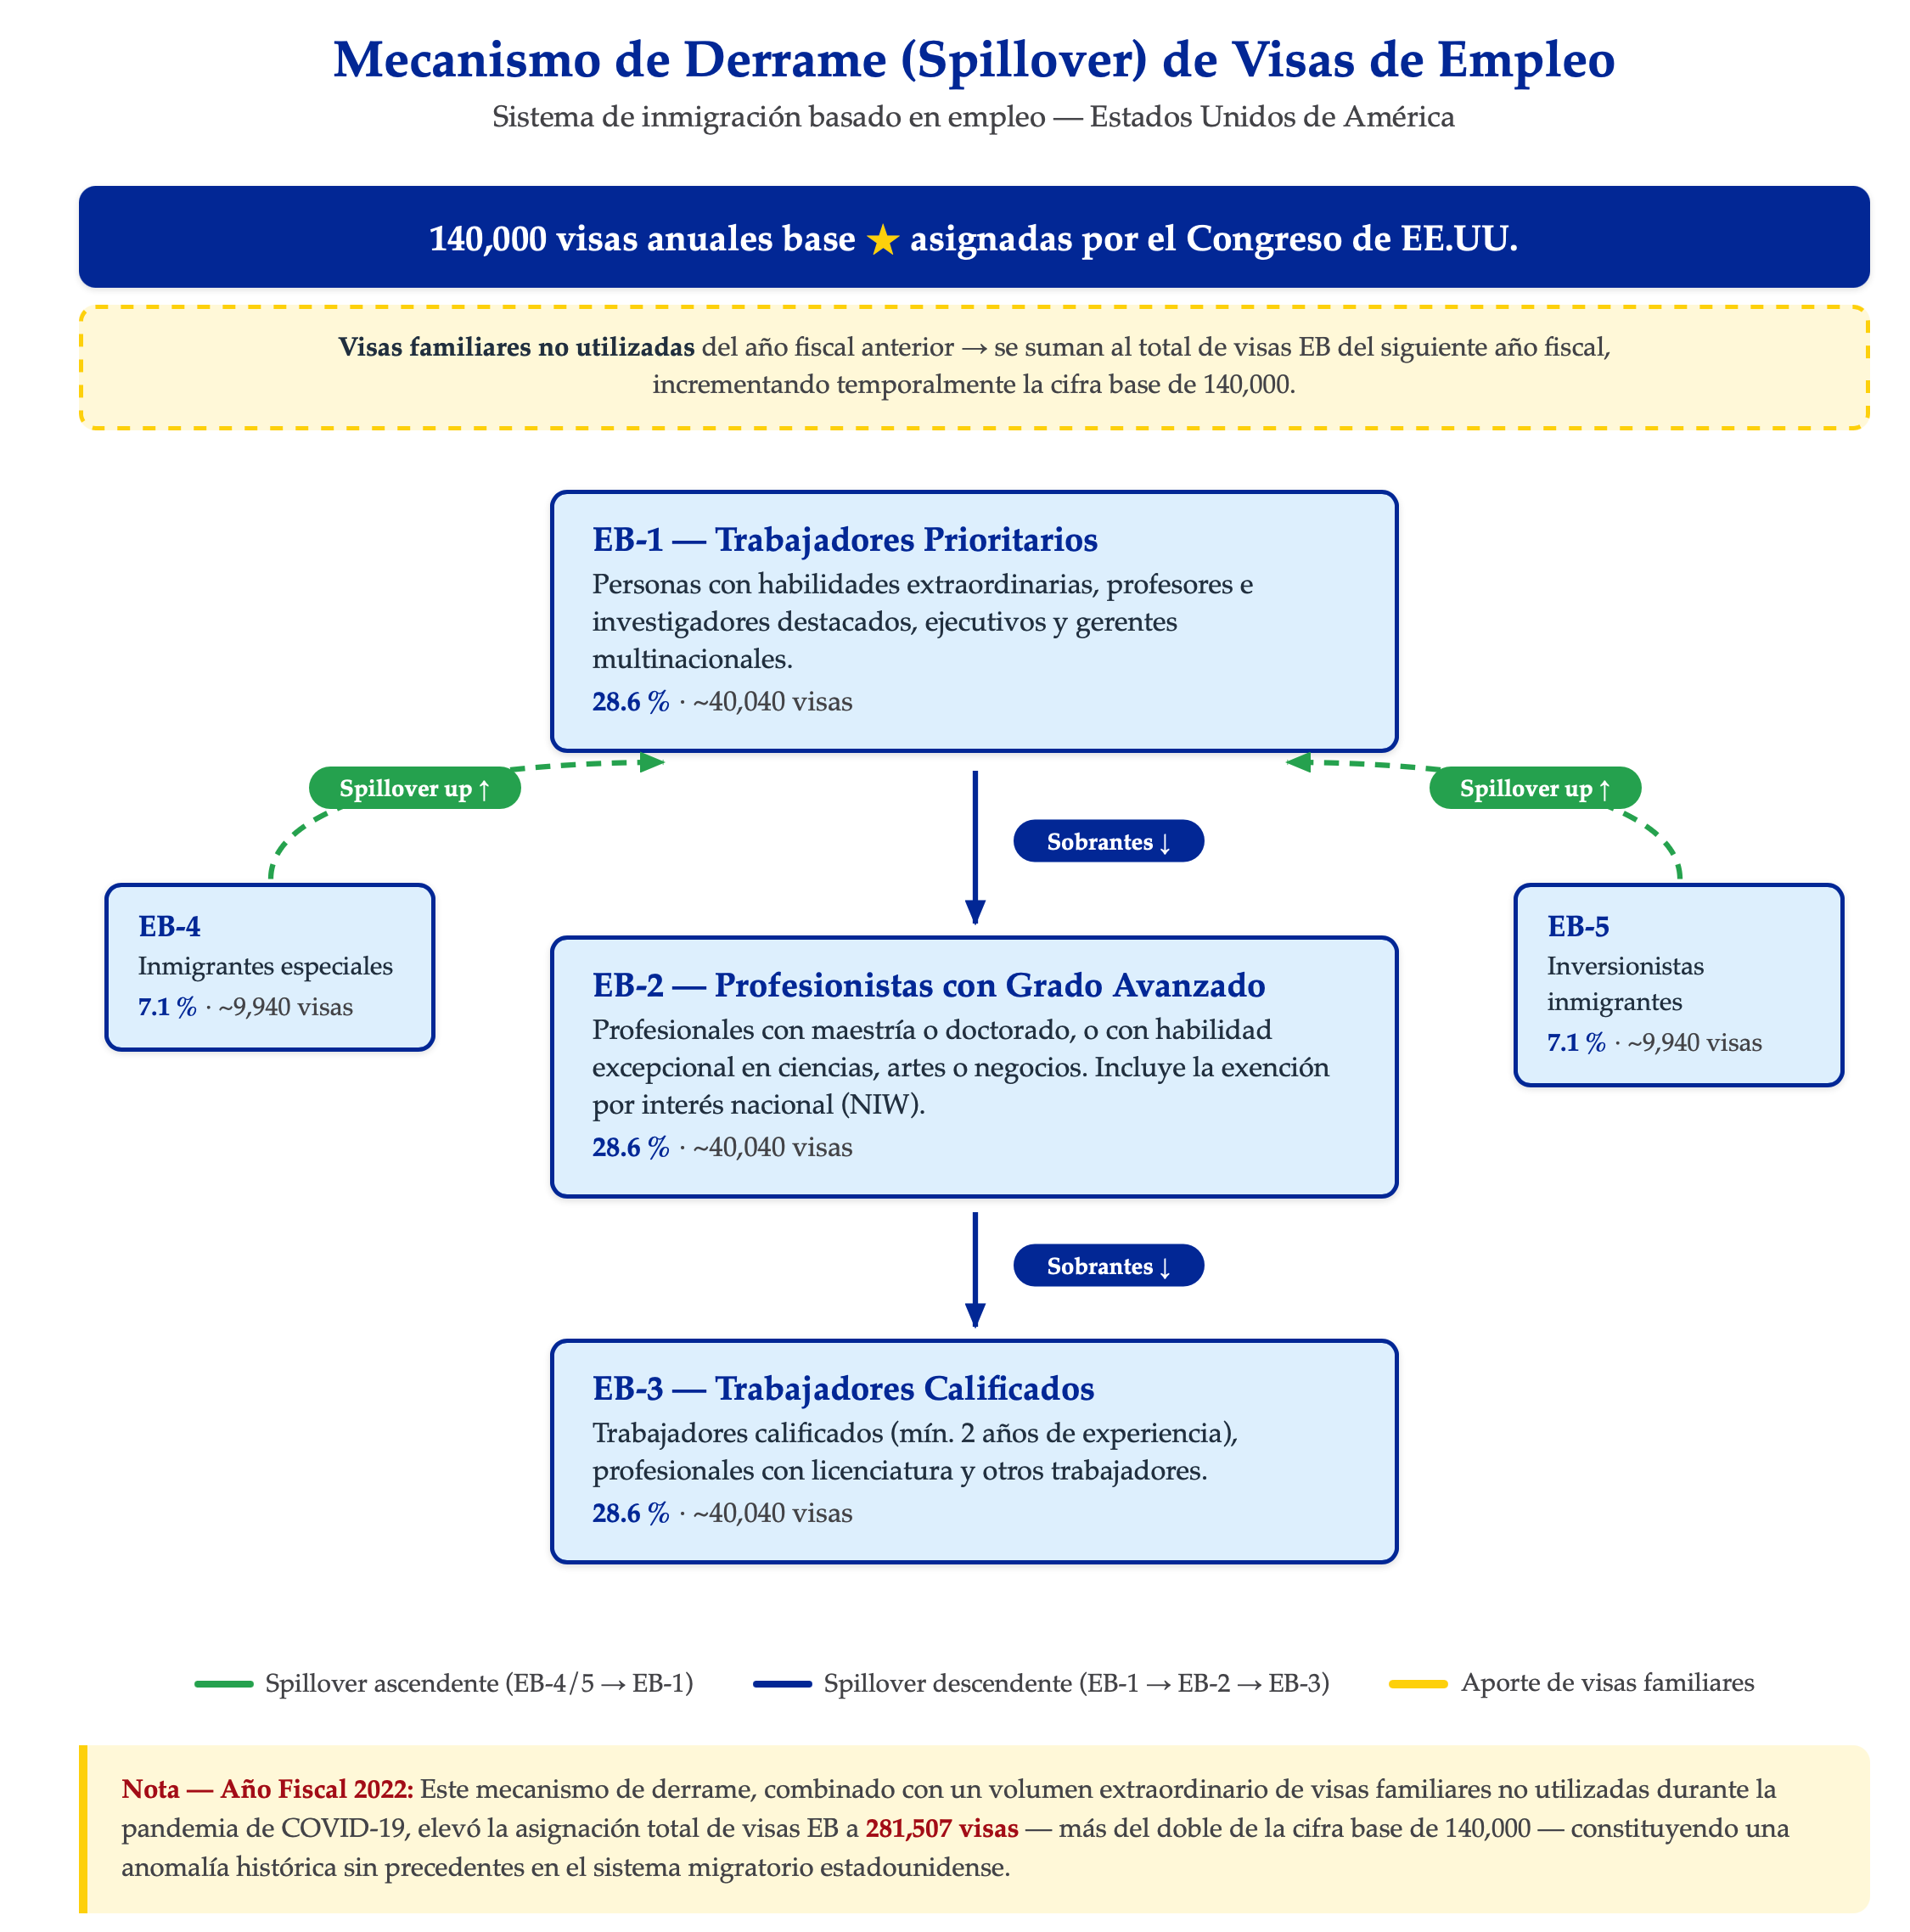
\includegraphics[width=1.0\textwidth]{spillover_diagram.png}
\caption{\footnotesize\color{uacjgray}\textit{Mecanismo de derrame (spillover) de visas entre categorías EB. Elaboración propia.}}
\label{fig:spillover}
\end{figure}

\subsection{¿Por qué este problema es computacionalmente difícil?}

La asignación de visas es estructuralmente equivalente a varios problemas conocidos como NP-Difícil \parencite{gareyjohnson1979}:

\begin{restrictionbox}
\textbf{Problema de Asignación Generalizada (GAP):} Asignar solicitantes (ítems) a espacios de visa (contenedores) con restricciones de capacidad heterogéneas.\\[4pt]
\textbf{Problema de Mochila Multidimensional:} Maximizar la utilización sujeta a restricciones de capacidad por país, por categoría y anual.\\[4pt]
\textbf{Programación de proyectos con recursos restringidos:} Asignar recursos escasos (números de visa) a actividades (solicitantes) con restricciones de precedencia (orden FIFO) y límites de capacidad.
\end{restrictionbox}

Tres características hacen que los métodos exactos sean \textbf{computacionalmente inviables}:

\textbf{(a) Integralidad.} Las visas son indivisibles. La relajación LP produce soluciones fraccionarias (e.g., asignar 0.3 visas) que requieren redondeo, violando restricciones o degradando significativamente la calidad.

\textbf{(b) Explosión combinatoria.} Con $\sim$1.8 millones de solicitantes, 200+ países, 5 categorías y 10+ años fiscales, el espacio de decisión tiene dimensionalidad del orden de \textbf{10,000+ dimensiones} con variables enteras.

\textbf{(c) Interacciones de restricciones no convexas.} El tope del 7\% por país crea \textit{efectos de acantilado} discontinuos: un país recibiendo 25,619 visas es factible, pero 25,621 no lo es. Las reglas de \textit{spillover} introducen restricciones condicionales que dependen de las asignaciones de otros países.

\begin{notebox}
\textbf{Conclusión de complejidad:} El método Simplex, los métodos de punto interior y los algoritmos basados en gradiente son inadecuados. Se requiere una metaheurística poblacional capaz de manejar restricciones enteras, no lineales y discontinuas en un contexto multiobjetivo.
\end{notebox}

\subsection{Formulación matemática del problema}

\subsubsection{Conjuntos e índices}

\begin{itemize}
    \item $\mathcal{I} = \{1, \ldots, N\}$: grupos de solicitantes (cohorte país-categoría-fecha de prioridad)
    \item $\mathcal{C} = \{1, \ldots, M\}$: países de carga (\textit{chargeability})
    \item $\mathcal{J} = \{1, \ldots, 5\}$: categorías de preferencia (EB-1 a EB-5)
    \item $\mathcal{T} = \{1, \ldots, H\}$: periodos de tiempo (años fiscales)
    \item $c(i)$: país del grupo $i$ \textcolor{uacjgray}{\textbullet} $j(i)$: categoría del grupo $i$
    \item $d_i$: fecha de prioridad del grupo $i$ \textcolor{uacjgray}{\textbullet} $n_i$: número de solicitantes en el grupo $i$
\end{itemize}

\subsubsection{Variables de decisión}

\begin{formulabox}
\begin{equation}
x_{i,t} \in \mathbb{Z}^+ : \text{número de visas asignadas al grupo } i \text{ en el periodo } t
\label{eq:decision}
\end{equation}
\end{formulabox}

Para la codificación en la metaheurística, se utiliza una \textbf{representación basada en permutación}: cada solución es una lista ordenada de grupos procesada por un decodificador greedy que asigna visas respetando todas las restricciones, garantizando factibilidad inherente.

\subsubsection{Funciones objetivo}

\textbf{Objetivo 1: Minimizar el tiempo promedio de espera.}

\begin{formulabox}
\begin{equation}
f_1(\mathbf{x}) = \frac{1}{N_{\text{total}}} \sum_{i \in \mathcal{I}} \sum_{t \in \mathcal{T}} x_{i,t} \cdot (t - d_i)
\label{eq:obj1}
\end{equation}
\end{formulabox}

\textbf{Objetivo 2: Maximizar la equidad (minimizar disparidad entre países).}

Se define el tiempo promedio de espera del país $c$:

\begin{formulabox}
\begin{equation}
\bar{W}_c(\mathbf{x}) = \frac{\displaystyle\sum_{i:\, c(i)=c}\; \sum_{t}\; x_{i,t} \cdot (t - d_i)}{\displaystyle\sum_{i:\, c(i)=c}\; n_i}
\label{eq:wait_country}
\end{equation}
\end{formulabox}

El objetivo minimax de equidad es:

\begin{formulabox}
\begin{equation}
f_2(\mathbf{x}) = \max_{c_1, c_2 \in \mathcal{C}} \left| \bar{W}_{c_1}(\mathbf{x}) - \bar{W}_{c_2}(\mathbf{x}) \right|
\label{eq:obj2}
\end{equation}
\end{formulabox}

\textbf{Objetivo 3: Maximizar la utilización de visas (minimizar desperdicio).}

\begin{formulabox}
\begin{equation}
f_3(\mathbf{x}) = \sum_{t \in \mathcal{T}} \left( V_t - \sum_{i \in \mathcal{I}} x_{i,t} \right)
\label{eq:obj3}
\end{equation}
\end{formulabox}

donde $V_t$ es el total de visas disponibles en el periodo $t$ ($\sim$140,000 base más \textit{spillover}).

\subsubsection{Restricciones}

\begin{table}[H]
\centering
\caption{Sistema de restricciones del problema de asignación de visas.}
\label{tab:restricciones}
\renewcommand{\arraystretch}{1.6}
\begin{tabular}{clp{7cm}}
\toprule
\rowcolor{tablehead}
\textcolor{white}{\textbf{ID}} & \textcolor{white}{\textbf{Restricción}} & \textcolor{white}{\textbf{Descripción}} \\
\midrule
C1 & $\displaystyle\sum_{i} x_{i,t} \leq V_t \;\; \forall t$ & Tope anual basado en empleo \\
\rowcolor{gray!8}
C2 & $\displaystyle\sum_{\substack{i:\\ c(i)=c}} x_{i,t} \leq 0.07 V_t^{\text{total}} \;\; \forall c, t$ & Tope por país del 7\% \\
C3 & $\displaystyle\sum_{\substack{i:\\ j(i)=j}} x_{i,t} \leq \text{Cap}_j(t) \;\; \forall j, t$ & Topes por categoría (incl. \textit{spillover}) \\
\rowcolor{gray!8}
C4 & FIFO por $(c, j)$ & Ordenamiento por fecha de prioridad \\
C5 & $\displaystyle\sum_t x_{i,t} \leq n_i \;\; \forall i$ & Restricción de demanda \\
\rowcolor{gray!8}
C6 & $x_{i,t} \in \mathbb{Z}^+ \;\; \forall i, t$ & No negatividad e integralidad \\
\bottomrule
\end{tabular}
\end{table}

\subsubsection{Conflicto entre objetivos}

\begin{figure}[H]
\centering
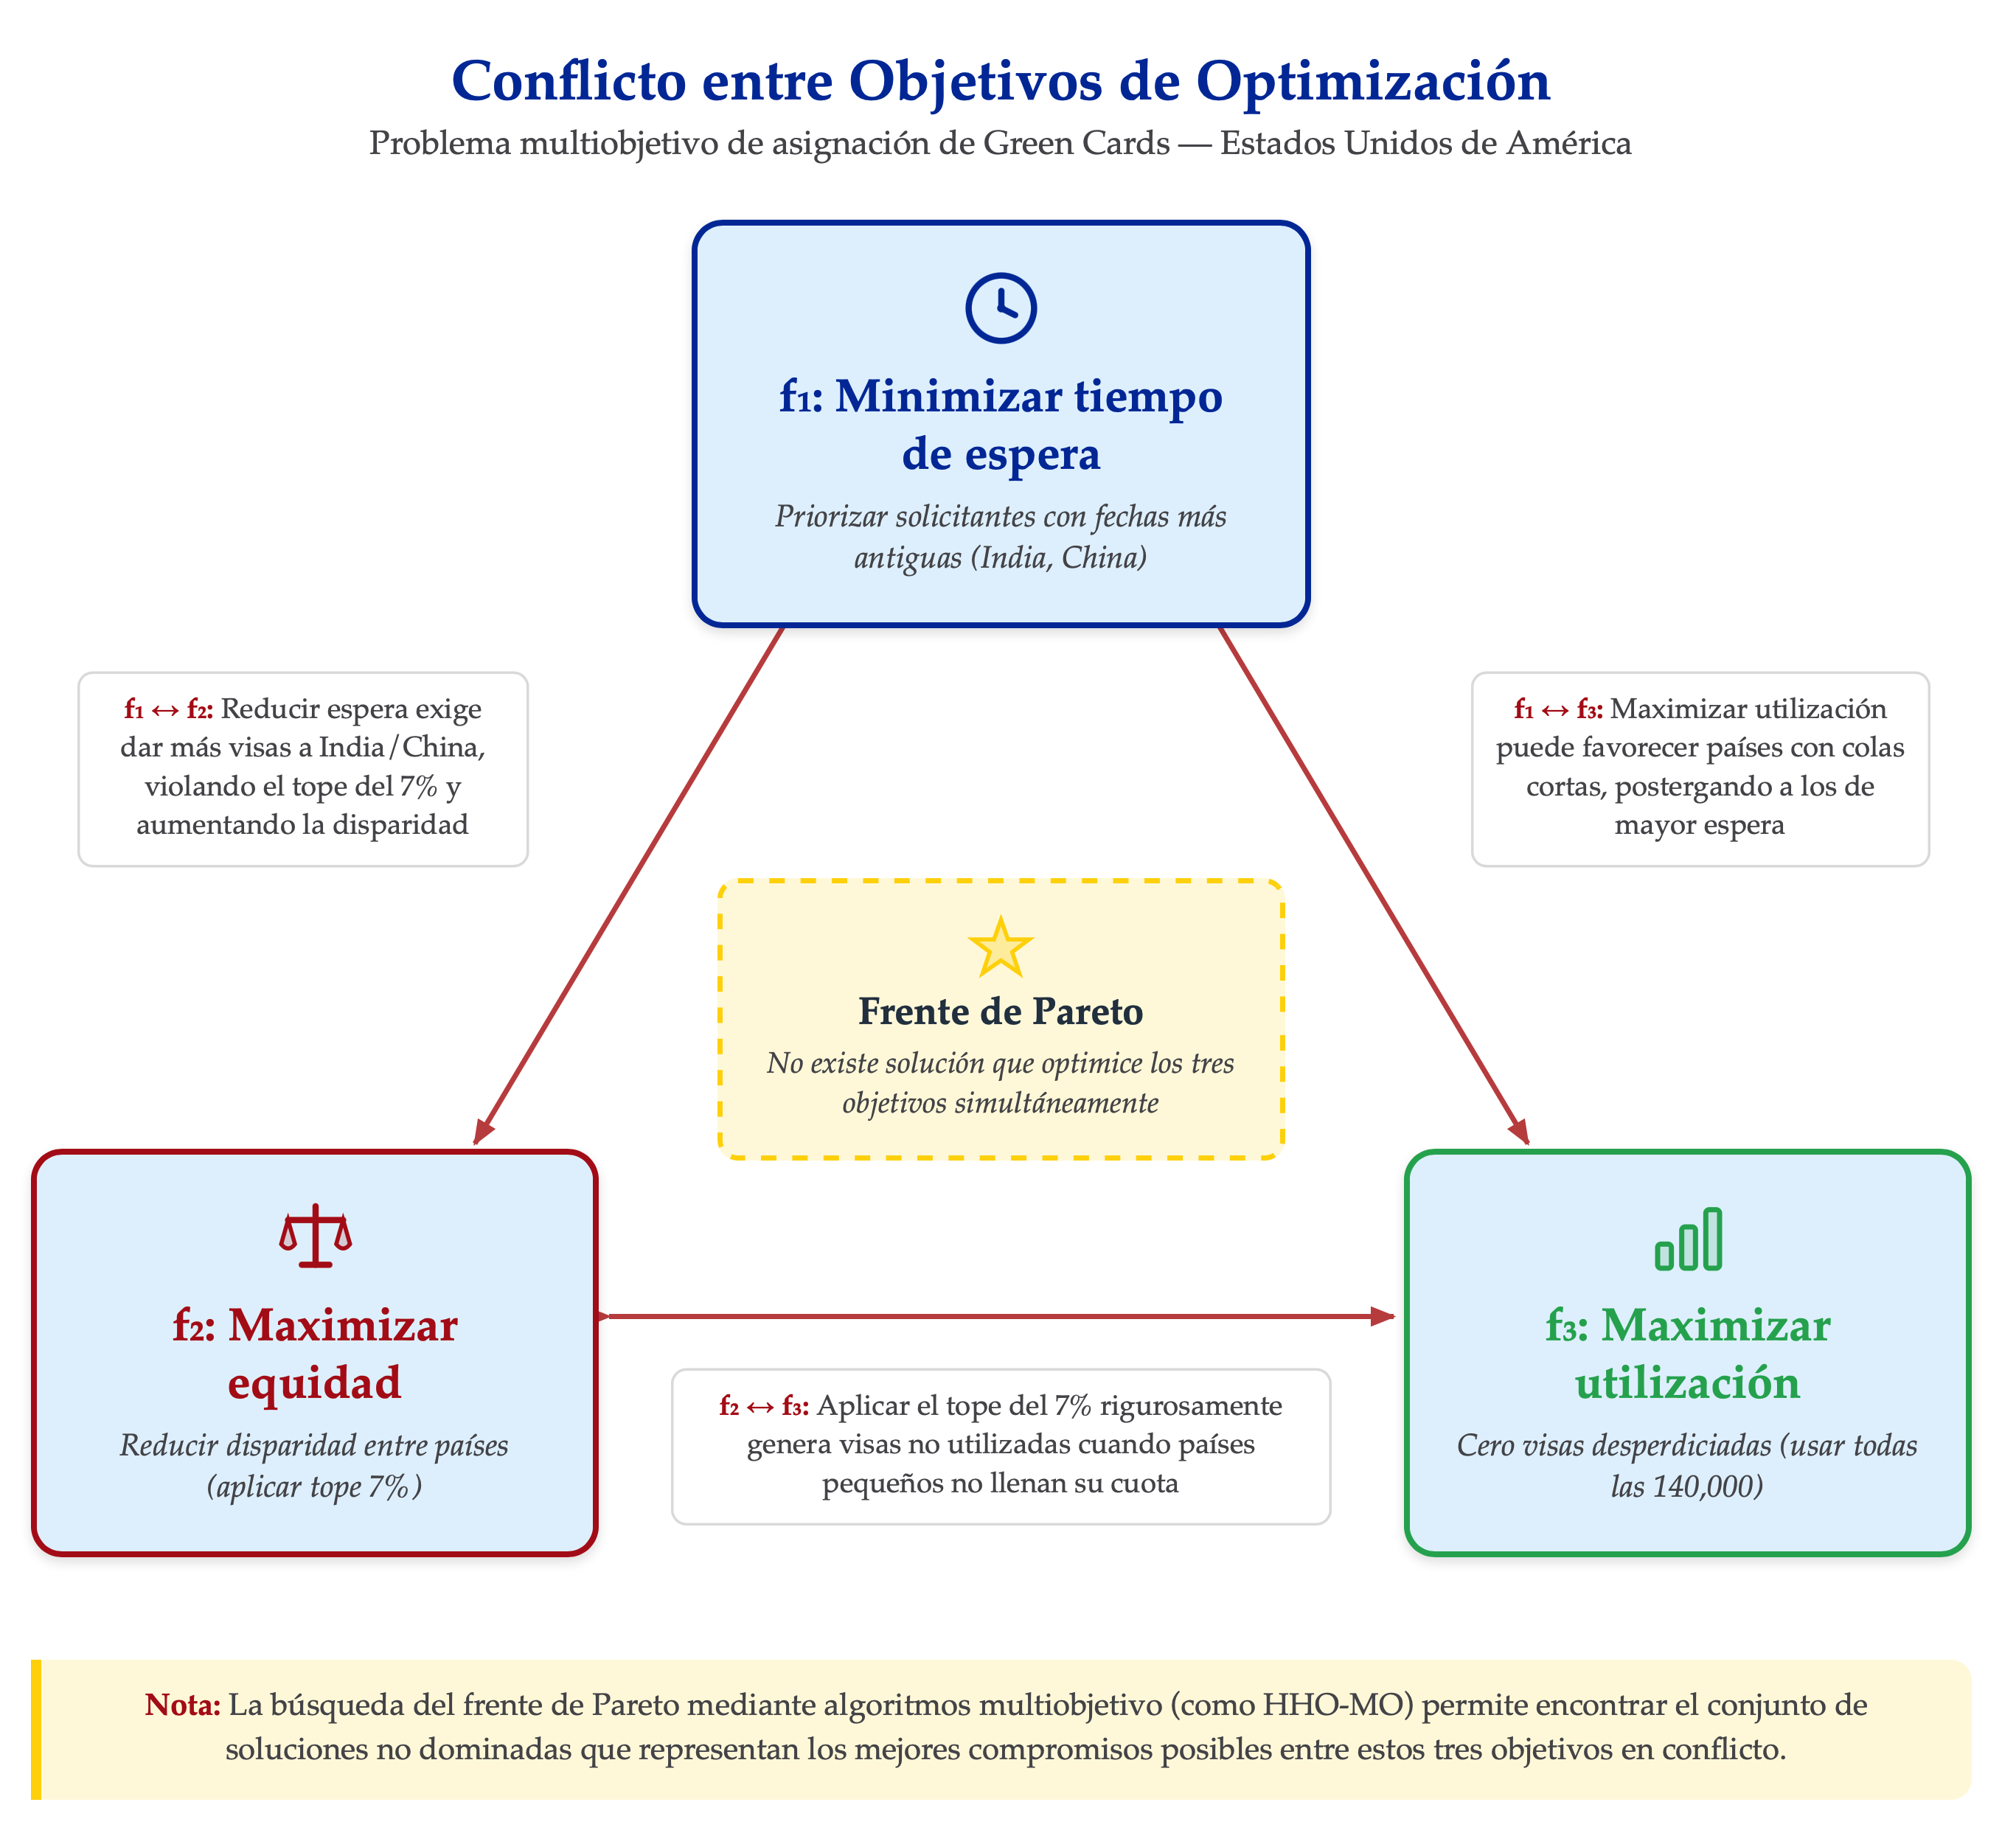
\includegraphics[width=1.0\textwidth]{conflicto_objetivos.png}
\caption{\footnotesize\color{uacjgray}\textit{Conflicto inherente entre los tres objetivos de optimización. Elaboración propia.}}
\label{fig:conflicto}
\end{figure}

Los tres objetivos entran en conflicto directo:

\textbf{$f_1$ vs. $f_2$:} Minimizar $f_1$ (tiempo de espera) exige asignar más visas a India y China, que tienen las fechas más antiguas. Pero hacerlo requiere relajar el tope del 7\%, lo que \textbf{incrementa} $f_2$ (disparidad).

\textbf{$f_2$ vs. $f_3$:} Aplicar el tope del 7\% rigurosamente (minimizando $f_2$) genera visas no utilizadas cuando países pequeños no pueden llenar su cuota, \textbf{incrementando} $f_3$ (desperdicio).

\textbf{$f_1$ vs. $f_3$:} Maximizar utilización ($f_3$) puede favorecer a solicitantes de países con colas cortas que están <<listos para procesar>>, postergando a solicitantes de larga espera, \textbf{empeorando} $f_1$.

\begin{yellowbox}
\textbf{Resultado clave:} No existe una asignación que optimice simultáneamente los tres objetivos. Esto convierte el problema en un genuino \textbf{problema de optimización de Pareto}, donde la solución es un \textit{frente} de asignaciones no dominadas que representan distintos compromisos (\textit{trade-offs}) entre eficiencia, equidad y utilización.
\end{yellowbox}


\begin{figure}[H]
\centering
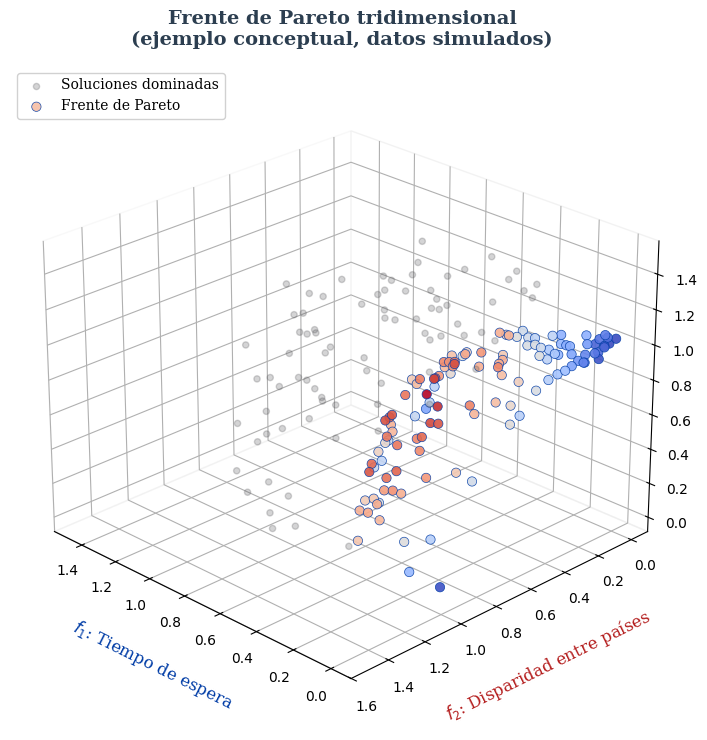
\includegraphics[width=0.85\textwidth]{pareto_front_3d.png}
\caption{\footnotesize\color{uacjgray}\textit{Ejemplo conceptual de un frente de Pareto tridimensional. Cada punto representa una asignación no dominada con diferentes compromisos entre $f_1$ (tiempo de espera), $f_2$ (equidad) y $f_3$ (utilización). El frente real se generará en la Fase Final del proyecto.}}
\label{fig:pareto}
\end{figure}

\subsection{Adaptación de HHO al contexto multiobjetivo (MOHHO)}

Para el problema multiobjetivo, se emplea la variante \textbf{MOHHO} (Multi-Objective Harris Hawks Optimizer), que incorpora tres elementos adicionales al HHO estándar \parencite{kusoglu2020, cerci2022}:

\textbf{(1) Archivo externo de Pareto.} Se reemplaza la <<presa>> única ($\mathbf{X}_{\text{rabbit}}$) por un \textbf{archivo externo} de soluciones no dominadas. Una solución $\mathbf{a}$ domina a $\mathbf{b}$ ($\mathbf{a} \succ \mathbf{b}$) si $\mathbf{a}$ es al menos igual en todos los objetivos y estrictamente mejor en al menos uno.

\textbf{(2) Selección de líder por distancia de aglomeración.} El <<conejo>> (líder) se selecciona del archivo mediante \textbf{ruleta ponderada por distancia de \textit{crowding}}:

\begin{formulabox}
\begin{equation}
CD(i) = \sum_{m=1}^{3} \frac{f_m(i+1) - f_m(i-1)}{f_m^{\max} - f_m^{\min}}
\label{eq:crowding}
\end{equation}
\end{formulabox}

Las soluciones en regiones menos pobladas del frente de Pareto tienen mayor probabilidad de ser seleccionadas como líderes, promoviendo diversidad.

\textbf{(3) Decodificador con reparación de restricciones.} Cada solución candidata (permutación de grupos) se decodifica de manera greedy: para cada grupo en el orden de la permutación, el decodificador verifica las restricciones C1 a C4 antes de asignar. Si alguna restricción se viola, el grupo se difiere al siguiente periodo. Esto \textbf{garantiza factibilidad} en toda solución decodificada.

% ==========================================================
% 8. IDONEIDAD DEL ALGORITMO
% ==========================================================
\section{¿Por qué HHO es Ideal para este Problema?}

Cinco propiedades del HHO se alinean con las características de la asignación de visas:

\textbf{(1) Intensidad de búsqueda adaptativa.} El parámetro $E$ proporciona una transición estocástica entre exploración y explotación. El paisaje de asignación contiene tanto mesetas amplias como crestas afiladas cerca de los límites por país. La intensidad oscilante de HHO navega ambas \parencite{heidari2019}.

\textbf{(2) Vuelos de Lévy para escapar de óptimos locales.} Los Operadores 5 y 6 generan saltos de largo alcance. En la asignación de visas, los óptimos locales surgen de las restricciones enteras y los topes por país.

\textbf{(3) Búsqueda cooperativa.} La población explora diversas regiones del espacio de asignación simultáneamente. Diferentes halcones pueden especializarse en distintas regiones del \textit{trade-off}.

\textbf{(4) Bajo conteo de parámetros.} Solo se requieren $N$ (población) y $T$ (iteraciones), lo cual minimiza la calibración necesaria.

\textbf{(5) Rendimiento combinatorio demostrado.} Variantes discretas de HHO han sido aplicadas exitosamente a selección de características, planificación de rutas, programación de trabajos y detección de comunidades \parencite{alabool2021, zhang2023}.

% ==========================================================
% 9. TRABAJO RELACIONADO
% ==========================================================
\section{Trabajo Relacionado}

Varios trabajos recientes aplican metodologías similares a problemas análogos de asignación con restricciones de equidad:

\textcite{pathak2025} formalizan la asignación de visas H-1B como un problema de diseño de reservas, demostrando que diferentes reglas pueden desplazar la asignación en 14,000 visas por año. \textcite{freund2023} desarrollan un marco de equidad grupal para la asignación dinámica de refugiados con \textit{trade-offs} casi idénticos a los de la asignación de visas. \textcite{bansak2024} extienden GeoMatch, un sistema de emparejamiento basado en ML para reasentamiento de refugiados con restricciones de capacidad, estructuralmente análogo a la asignación de visas con topes por país. \textcite{li2024fairness} proporcionan un estudio exhaustivo sobre la incorporación de equidad en la optimización multiobjetivo, discutiendo eficiencia equitativa y el principio de Pigou-Dalton, directamente aplicable al objetivo $f_2$.

% ==========================================================
% 10. TRABAJO FUTURO
% ==========================================================
\section{Trabajo Futuro: Fases 02 y Final}

En la \textbf{segunda evaluación parcial}, se desarrollará el modelo matemático completo, incluyendo la formulación formal con datos reales del \textit{Visa Bulletin} y la estrategia de integración del modelo con MOHHO.

En la \textbf{evaluación final}, se implementará MOHHO en Python, se realizará experimentación controlada con datos reales de demanda por país y categoría, y se analizará el frente de Pareto resultante. Se compararán los resultados contra la asignación actual del sistema y, si el tiempo lo permite, contra NSGA-II como \textit{baseline}.


\newpage
% ==========================================================
% 11. CONCLUSIONES
% ==========================================================
\section{Conclusiones y Reflexiones Finales}

\subsection{Conclusiones}

Este proyecto demuestra que la asignación de Green Cards en Estados Unidos constituye un problema de optimización multiobjetivo combinatorio de alta complejidad (NP-Difícil), con restricciones no lineales y discontinuas que hacen inviables los métodos exactos. El algoritmo HHO, con sus seis operadores y su mecanismo de energía adaptativa, ofrece una arquitectura rica y flexible para explorar el frente de Pareto de soluciones que equilibren tiempo de espera, equidad y utilización.

La selección de HHO cumple con todos los requisitos del proyecto: es una metaheurística moderna (2019), no cubierta en el temario, con extensiones multiobjetivo validadas y aplicaciones combinatorias demostradas. El problema elegido no solo tiene rigor académico; tiene urgencia humana.

\subsection{Yazmín Flores - Relfexión}


\begin{wrapfigure}{l}{3cm}
     \vspace{-0.3cm}
     \centering
     
\includegraphics[width=2.8cm]{yazmin_photo.jpg}
     \vspace{-0.3cm}
\end{wrapfigure}

Llegué a Estados Unidos en 2012. Años de incertidumbre, formularios y el miedo constante a que un cambio de administración borre años de espera. Mi proceso finalmente resultó positivo: obtuve mi Green Card. Pero el alivio vino acompañado de una pregunta que no me ha dejado: \textbf{¿por qué tuvo que ser así?} Cada variable $x_{i,t}$ en este modelo representa a una persona real.

\subsection{Javier Rebull - Reflexión}

\begin{wrapfigure}{l}{3cm}
    \vspace{-0.3cm}
    \centering
    
\includegraphics[width=2.8cm]{javi_photo.jpg}
    \vspace{-0.3cm}
\end{wrapfigure}

Vivo en Boston desde 2013. He pasado por \textbf{dos procesos de Green Card fallidos}: el primero interrumpido por un cambio de empleador, el segundo atrapado en el procesamiento USCIS durante COVID. Hoy sigo esperando. Elegimos este problema porque es \textbf{nuestro problema}. Los halcones de Harris cazan en equipo porque un halcón solo no puede atrapar un conejo que zigzaguea: los problemas complejos requieren cooperación, adaptación y persistencia.

\vspace{1.5em}
{\color{uacjgray}\hrule}
\vspace{1em}


% ==========================================================
% REFERENCIAS
% ==========================================================
\newpage
\begingroup
\emergencystretch=2em
\printbibliography[title={Referencias}]
\endgroup

\end{document}